% Options for packages loaded elsewhere
\PassOptionsToPackage{unicode}{hyperref}
\PassOptionsToPackage{hyphens}{url}
\PassOptionsToPackage{dvipsnames,svgnames,x11names}{xcolor}
%
\documentclass[
  letterpaper,
  DIV=11,
  numbers=noendperiod]{scrreprt}

\usepackage{amsmath,amssymb}
\usepackage{lmodern}
\usepackage{iftex}
\ifPDFTeX
  \usepackage[T1]{fontenc}
  \usepackage[utf8]{inputenc}
  \usepackage{textcomp} % provide euro and other symbols
\else % if luatex or xetex
  \usepackage{unicode-math}
  \defaultfontfeatures{Scale=MatchLowercase}
  \defaultfontfeatures[\rmfamily]{Ligatures=TeX,Scale=1}
\fi
% Use upquote if available, for straight quotes in verbatim environments
\IfFileExists{upquote.sty}{\usepackage{upquote}}{}
\IfFileExists{microtype.sty}{% use microtype if available
  \usepackage[]{microtype}
  \UseMicrotypeSet[protrusion]{basicmath} % disable protrusion for tt fonts
}{}
\makeatletter
\@ifundefined{KOMAClassName}{% if non-KOMA class
  \IfFileExists{parskip.sty}{%
    \usepackage{parskip}
  }{% else
    \setlength{\parindent}{0pt}
    \setlength{\parskip}{6pt plus 2pt minus 1pt}}
}{% if KOMA class
  \KOMAoptions{parskip=half}}
\makeatother
\usepackage{xcolor}
\setlength{\emergencystretch}{3em} % prevent overfull lines
\setcounter{secnumdepth}{5}
% Make \paragraph and \subparagraph free-standing
\ifx\paragraph\undefined\else
  \let\oldparagraph\paragraph
  \renewcommand{\paragraph}[1]{\oldparagraph{#1}\mbox{}}
\fi
\ifx\subparagraph\undefined\else
  \let\oldsubparagraph\subparagraph
  \renewcommand{\subparagraph}[1]{\oldsubparagraph{#1}\mbox{}}
\fi

\usepackage{color}
\usepackage{fancyvrb}
\newcommand{\VerbBar}{|}
\newcommand{\VERB}{\Verb[commandchars=\\\{\}]}
\DefineVerbatimEnvironment{Highlighting}{Verbatim}{commandchars=\\\{\}}
% Add ',fontsize=\small' for more characters per line
\usepackage{framed}
\definecolor{shadecolor}{RGB}{241,243,245}
\newenvironment{Shaded}{\begin{snugshade}}{\end{snugshade}}
\newcommand{\AlertTok}[1]{\textcolor[rgb]{0.68,0.00,0.00}{#1}}
\newcommand{\AnnotationTok}[1]{\textcolor[rgb]{0.37,0.37,0.37}{#1}}
\newcommand{\AttributeTok}[1]{\textcolor[rgb]{0.40,0.45,0.13}{#1}}
\newcommand{\BaseNTok}[1]{\textcolor[rgb]{0.68,0.00,0.00}{#1}}
\newcommand{\BuiltInTok}[1]{\textcolor[rgb]{0.00,0.23,0.31}{#1}}
\newcommand{\CharTok}[1]{\textcolor[rgb]{0.13,0.47,0.30}{#1}}
\newcommand{\CommentTok}[1]{\textcolor[rgb]{0.37,0.37,0.37}{#1}}
\newcommand{\CommentVarTok}[1]{\textcolor[rgb]{0.37,0.37,0.37}{\textit{#1}}}
\newcommand{\ConstantTok}[1]{\textcolor[rgb]{0.56,0.35,0.01}{#1}}
\newcommand{\ControlFlowTok}[1]{\textcolor[rgb]{0.00,0.23,0.31}{#1}}
\newcommand{\DataTypeTok}[1]{\textcolor[rgb]{0.68,0.00,0.00}{#1}}
\newcommand{\DecValTok}[1]{\textcolor[rgb]{0.68,0.00,0.00}{#1}}
\newcommand{\DocumentationTok}[1]{\textcolor[rgb]{0.37,0.37,0.37}{\textit{#1}}}
\newcommand{\ErrorTok}[1]{\textcolor[rgb]{0.68,0.00,0.00}{#1}}
\newcommand{\ExtensionTok}[1]{\textcolor[rgb]{0.00,0.23,0.31}{#1}}
\newcommand{\FloatTok}[1]{\textcolor[rgb]{0.68,0.00,0.00}{#1}}
\newcommand{\FunctionTok}[1]{\textcolor[rgb]{0.28,0.35,0.67}{#1}}
\newcommand{\ImportTok}[1]{\textcolor[rgb]{0.00,0.46,0.62}{#1}}
\newcommand{\InformationTok}[1]{\textcolor[rgb]{0.37,0.37,0.37}{#1}}
\newcommand{\KeywordTok}[1]{\textcolor[rgb]{0.00,0.23,0.31}{#1}}
\newcommand{\NormalTok}[1]{\textcolor[rgb]{0.00,0.23,0.31}{#1}}
\newcommand{\OperatorTok}[1]{\textcolor[rgb]{0.37,0.37,0.37}{#1}}
\newcommand{\OtherTok}[1]{\textcolor[rgb]{0.00,0.23,0.31}{#1}}
\newcommand{\PreprocessorTok}[1]{\textcolor[rgb]{0.68,0.00,0.00}{#1}}
\newcommand{\RegionMarkerTok}[1]{\textcolor[rgb]{0.00,0.23,0.31}{#1}}
\newcommand{\SpecialCharTok}[1]{\textcolor[rgb]{0.37,0.37,0.37}{#1}}
\newcommand{\SpecialStringTok}[1]{\textcolor[rgb]{0.13,0.47,0.30}{#1}}
\newcommand{\StringTok}[1]{\textcolor[rgb]{0.13,0.47,0.30}{#1}}
\newcommand{\VariableTok}[1]{\textcolor[rgb]{0.07,0.07,0.07}{#1}}
\newcommand{\VerbatimStringTok}[1]{\textcolor[rgb]{0.13,0.47,0.30}{#1}}
\newcommand{\WarningTok}[1]{\textcolor[rgb]{0.37,0.37,0.37}{\textit{#1}}}

\providecommand{\tightlist}{%
  \setlength{\itemsep}{0pt}\setlength{\parskip}{0pt}}\usepackage{longtable,booktabs,array}
\usepackage{calc} % for calculating minipage widths
% Correct order of tables after \paragraph or \subparagraph
\usepackage{etoolbox}
\makeatletter
\patchcmd\longtable{\par}{\if@noskipsec\mbox{}\fi\par}{}{}
\makeatother
% Allow footnotes in longtable head/foot
\IfFileExists{footnotehyper.sty}{\usepackage{footnotehyper}}{\usepackage{footnote}}
\makesavenoteenv{longtable}
\usepackage{graphicx}
\makeatletter
\def\maxwidth{\ifdim\Gin@nat@width>\linewidth\linewidth\else\Gin@nat@width\fi}
\def\maxheight{\ifdim\Gin@nat@height>\textheight\textheight\else\Gin@nat@height\fi}
\makeatother
% Scale images if necessary, so that they will not overflow the page
% margins by default, and it is still possible to overwrite the defaults
% using explicit options in \includegraphics[width, height, ...]{}
\setkeys{Gin}{width=\maxwidth,height=\maxheight,keepaspectratio}
% Set default figure placement to htbp
\makeatletter
\def\fps@figure{htbp}
\makeatother
\newlength{\cslhangindent}
\setlength{\cslhangindent}{1.5em}
\newlength{\csllabelwidth}
\setlength{\csllabelwidth}{3em}
\newlength{\cslentryspacingunit} % times entry-spacing
\setlength{\cslentryspacingunit}{\parskip}
\newenvironment{CSLReferences}[2] % #1 hanging-ident, #2 entry spacing
 {% don't indent paragraphs
  \setlength{\parindent}{0pt}
  % turn on hanging indent if param 1 is 1
  \ifodd #1
  \let\oldpar\par
  \def\par{\hangindent=\cslhangindent\oldpar}
  \fi
  % set entry spacing
  \setlength{\parskip}{#2\cslentryspacingunit}
 }%
 {}
\usepackage{calc}
\newcommand{\CSLBlock}[1]{#1\hfill\break}
\newcommand{\CSLLeftMargin}[1]{\parbox[t]{\csllabelwidth}{#1}}
\newcommand{\CSLRightInline}[1]{\parbox[t]{\linewidth - \csllabelwidth}{#1}\break}
\newcommand{\CSLIndent}[1]{\hspace{\cslhangindent}#1}

\KOMAoption{captions}{tableheading}
\makeatletter
\@ifpackageloaded{tcolorbox}{}{\usepackage[many]{tcolorbox}}
\@ifpackageloaded{fontawesome5}{}{\usepackage{fontawesome5}}
\definecolor{quarto-callout-color}{HTML}{909090}
\definecolor{quarto-callout-note-color}{HTML}{0758E5}
\definecolor{quarto-callout-important-color}{HTML}{CC1914}
\definecolor{quarto-callout-warning-color}{HTML}{EB9113}
\definecolor{quarto-callout-tip-color}{HTML}{00A047}
\definecolor{quarto-callout-caution-color}{HTML}{FC5300}
\definecolor{quarto-callout-color-frame}{HTML}{acacac}
\definecolor{quarto-callout-note-color-frame}{HTML}{4582ec}
\definecolor{quarto-callout-important-color-frame}{HTML}{d9534f}
\definecolor{quarto-callout-warning-color-frame}{HTML}{f0ad4e}
\definecolor{quarto-callout-tip-color-frame}{HTML}{02b875}
\definecolor{quarto-callout-caution-color-frame}{HTML}{fd7e14}
\makeatother
\makeatletter
\makeatother
\makeatletter
\@ifpackageloaded{bookmark}{}{\usepackage{bookmark}}
\makeatother
\makeatletter
\@ifpackageloaded{caption}{}{\usepackage{caption}}
\AtBeginDocument{%
\ifdefined\contentsname
  \renewcommand*\contentsname{Table of contents}
\else
  \newcommand\contentsname{Table of contents}
\fi
\ifdefined\listfigurename
  \renewcommand*\listfigurename{List of Figures}
\else
  \newcommand\listfigurename{List of Figures}
\fi
\ifdefined\listtablename
  \renewcommand*\listtablename{List of Tables}
\else
  \newcommand\listtablename{List of Tables}
\fi
\ifdefined\figurename
  \renewcommand*\figurename{Figure}
\else
  \newcommand\figurename{Figure}
\fi
\ifdefined\tablename
  \renewcommand*\tablename{Table}
\else
  \newcommand\tablename{Table}
\fi
}
\@ifpackageloaded{float}{}{\usepackage{float}}
\floatstyle{ruled}
\@ifundefined{c@chapter}{\newfloat{codelisting}{h}{lop}}{\newfloat{codelisting}{h}{lop}[chapter]}
\floatname{codelisting}{Listing}
\newcommand*\listoflistings{\listof{codelisting}{List of Listings}}
\usepackage{amsthm}
\theoremstyle{definition}
\newtheorem{example}{Example}[chapter]
\theoremstyle{remark}
\renewcommand*{\proofname}{Proof}
\newtheorem*{remark}{Remark}
\newtheorem*{solution}{Solution}
\makeatother
\makeatletter
\@ifpackageloaded{caption}{}{\usepackage{caption}}
\@ifpackageloaded{subcaption}{}{\usepackage{subcaption}}
\makeatother
\makeatletter
\@ifpackageloaded{tcolorbox}{}{\usepackage[many]{tcolorbox}}
\makeatother
\makeatletter
\@ifundefined{shadecolor}{\definecolor{shadecolor}{rgb}{.97, .97, .97}}
\makeatother
\makeatletter
\makeatother
\ifLuaTeX
  \usepackage{selnolig}  % disable illegal ligatures
\fi
\IfFileExists{bookmark.sty}{\usepackage{bookmark}}{\usepackage{hyperref}}
\IfFileExists{xurl.sty}{\usepackage{xurl}}{} % add URL line breaks if available
\urlstyle{same} % disable monospaced font for URLs
\hypersetup{
  pdftitle={Part II Computational Physics},
  pdfauthor={Austen Lamacraft},
  colorlinks=true,
  linkcolor={blue},
  filecolor={Maroon},
  citecolor={Blue},
  urlcolor={Blue},
  pdfcreator={LaTeX via pandoc}}

\title{Part II Computational Physics}
\author{Austen Lamacraft}
\date{1/17/23}

\begin{document}
\maketitle
\ifdefined\Shaded\renewenvironment{Shaded}{\begin{tcolorbox}[interior hidden, frame hidden, breakable, enhanced, boxrule=0pt, sharp corners, borderline west={3pt}{0pt}{shadecolor}]}{\end{tcolorbox}}\fi

\renewcommand*\contentsname{Table of contents}
{
\hypersetup{linkcolor=}
\setcounter{tocdepth}{2}
\tableofcontents
}
\bookmarksetup{startatroot}

\hypertarget{preface}{%
\chapter*{Preface}\label{preface}}
\addcontentsline{toc}{chapter}{Preface}

\markboth{Preface}{Preface}

These are the materials for the Part II Physics course Computational
Physics, taught in Lent Term 2023 at the University of Cambridge.

\hypertarget{schedule}{%
\section*{Schedule}\label{schedule}}
\addcontentsline{toc}{section}{Schedule}

\markright{Schedule}

The course of eight Lectures will take place at 10.00 on Mondays and
Fridays in the Pippard Lecture Theatre. After the lectures there will be
four computing exercises to be completed in the last four weeks of full
Lent term; one per week. Remember that the exercises count for 0.2 units
or further work, or roughly 2\% of your final mark for the year. Thus
each exercise should only take you a few hours.

The schedule is as follows

\begin{itemize}
\tightlist
\item
  First lecture: Monday 23th January
\item
  Last lecture: Friday 17th February
\item
  First exercise: Friday 17th February -- Friday 24th February
\item
  Second exercise: Friday 24th February -- Friday 3rd March
\item
  Third exercise: Friday 3rd March -- Friday 10th March
\item
  Fourth exercise: Friday 10th March -- Friday 17th March (last day of
  full Lent term)
\end{itemize}

\hypertarget{prerequisites}{%
\section*{Prerequisites}\label{prerequisites}}
\addcontentsline{toc}{section}{Prerequisites}

\markright{Prerequisites}

This course assumes a basic knowledge of the Python language, including
variables, control flow, and writing and using functions, at the level
of last year's IB course.

\hypertarget{learning-outcomes}{%
\section*{Learning outcomes}\label{learning-outcomes}}
\addcontentsline{toc}{section}{Learning outcomes}

\markright{Learning outcomes}

In this course you will learn

\begin{enumerate}
\def\labelenumi{\arabic{enumi}.}
\tightlist
\item
  About the Python scientific stack (based on the NumPy library)
\item
  Its use in implementing some common algorithms in computational
  physics.
\item
  Basic ideas of computational complexity used in the analysis of
  algorithms
\end{enumerate}

\hypertarget{outline}{%
\section*{Outline}\label{outline}}
\addcontentsline{toc}{section}{Outline}

\markright{Outline}

Here's a list of topics that I'd like to cover. We make not have time
for all of them.

\begin{enumerate}
\def\labelenumi{\arabic{enumi}.}
\tightlist
\item
  Setup. Running Python. Notebooks. Language overview
\item
  NumPy and friends
\item
  Floating point and all that
\item
  Soving differential equations with SciPy
\item
  Monte Carlo methods
\item
  Linear algebra with NumPy
\item
  Introduction to algorithms and complexity
\item
  The fast Fourier transform
\item
  Automatic differentiation
\end{enumerate}

\hypertarget{these-notes}{%
\section*{These notes\ldots{}}\label{these-notes}}
\addcontentsline{toc}{section}{These notes\ldots{}}

\markright{These notes\ldots{}}

\ldots were prepared using \href{https://quarto.org/}{Quarto}. Each
chapter should be thought of as a Jupyter notebook (actually, they
\emph{are} Jupyter notebooks), so you'll only see
\texttt{import\ numpy\ as\ np} once in each chapter, for example.

In several places I've used examples from an earlier version of the
course by David Buscher.

\bookmarksetup{startatroot}

\hypertarget{introduction}{%
\chapter{Introduction}\label{introduction}}

\begin{quote}
Science is what we understand well enough to explain to a computer. Art
is everything else we do.

Donald Knuth
\end{quote}

Not a course on numerical analysis but computational physics

Computation is important for experimental physicists for analysing data.
For theoretical physics, computation is used to deal with the awkward
fact that physical theories are \emph{generally not tractable}. You
can't solve Maxwell's equations, the Navier--Stokes equation, or
Schrödinger's equation in any but the simplest situations.

To be blunt, this means that your knowledge of physics, while very nice,
is of \emph{no use whatsoever} unless you can write a program to solve
more complicated problems. Sorry.

It's important to understand that this need to apply our mathematical
descriptions of nature in more general settings was the principal
driving force behind the invention of the computer.

More than this,

Church Turing hypothesis

Turing's cathedral

Books

Part IB notes are very good

Garth Wells

https://github.com/CambridgeEngineering/PartIA-Computing-Michaelmas/

Rougier

https://www.labri.fr/perso/nrougier/from-python-to-numpy/
https://github.com/rougier/scientific-visualization-book

\bookmarksetup{startatroot}

\hypertarget{getting-going}{%
\chapter{Getting Going}\label{getting-going}}

\hypertarget{finding-your-way}{%
\section{Finding your way}\label{finding-your-way}}

Everyone finds their own workflow for coding, depending on their
preferred language, editor, how they run their code, and so on. The aim
of the sections below is to give a roundup of some popular tools in the
Python ecosystem.

\hypertarget{your-coding-environment}{%
\section{Your coding environment}\label{your-coding-environment}}

To run Python code on your computer you will need to have installed the
Python language. I recommend the
\href{https://www.anaconda.com/products/distribution}{Anaconda
distribution} as it comes with all the parts of the toolkit we'll need
such as \href{https://jupyter.org/}{Jupyter notebooks} and the major
libraries \href{https://numpy.org/}{NumPy} and
\href{https://scipy.org/}{SciPy}.

Try running \texttt{python} at the command line. You should get
something like

\begin{verbatim}
Python 3.9.12 (main, Apr  5 2022, 01:53:17) 
[Clang 12.0.0 ] :: Anaconda, Inc. on darwin
Type "help", "copyright", "credits" or "license" for more information.
>>> 
\end{verbatim}

You should confirm that you are using Python 3 (the command
\texttt{python3} will also work and guarantee this if you happen to have
Python 2 as the default). The prompt
\texttt{\textgreater{}\textgreater{}\textgreater{}} indicates that you
have started the Python interactive shell or
\href{https://en.wikipedia.org/wiki/Read\%E2\%80\%93eval\%E2\%80\%93print_loop}{REPL}
and are good to go:

\begin{Shaded}
\begin{Highlighting}[]
\BuiltInTok{print}\NormalTok{(}\StringTok{"Hello world!"}\NormalTok{)}
\DecValTok{1} \OperatorTok{+} \DecValTok{2}
\end{Highlighting}
\end{Shaded}

\begin{verbatim}
Hello world!
\end{verbatim}

\begin{verbatim}
3
\end{verbatim}

To leave and return to the command line, you can run \texttt{quit()} or
\texttt{exit()}.

\hypertarget{ipython}{%
\section{IPython}\label{ipython}}

If you ran the above command from within \texttt{python} you may have
noticed that the nice colour scheme that you see above was absent. This
is called
\href{https://en.wikipedia.org/wiki/Syntax_highlighting}{syntax
highlighting} and provides a visual guide to the syntax of the language.

\href{https://ipython.readthedocs.io/en/stable/}{IPython} is an
interactive shell that provides syntax highlighting and much more. If
you have installed IPython (it comes with Anaconda) you can start it
from the command line with \texttt{ipython}.

Among the most helpful features of IPython are:

\begin{enumerate}
\def\labelenumi{\arabic{enumi}.}
\tightlist
\item
  Tab completion: hit \texttt{tab} to autocomplete. This is particularly
  useful for viewing all properties or methods of an object:
  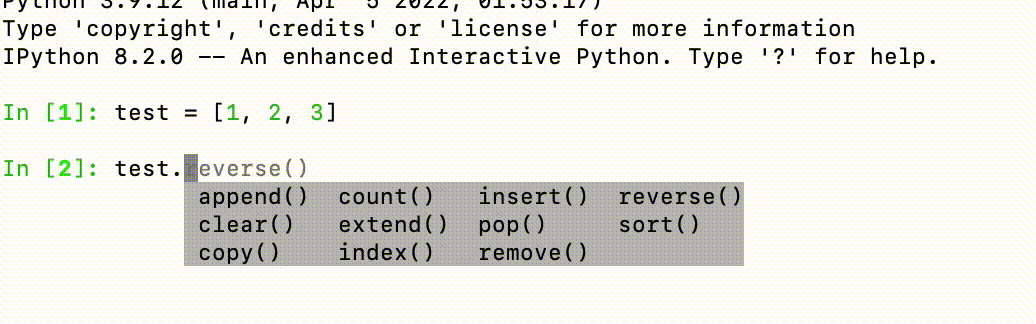
\includegraphics{./assets/tab-complete.png}
\item
  Typing \texttt{?word} or \texttt{word?} prints detailed information
  about an object (\texttt{??} provides additional detail).
\item
  Certain \emph{magic commands} prefixed by \texttt{\%} that provide
  certain additional functionality. For example, \texttt{\%timeit} finds
  the executation time of a single line statement, which is useful when
  profiling the performance of code:
\end{enumerate}

\begin{Shaded}
\begin{Highlighting}[]
\OperatorTok{\%}\NormalTok{timeit L }\OperatorTok{=}\NormalTok{ [n }\OperatorTok{**} \DecValTok{2} \ControlFlowTok{for}\NormalTok{ n }\KeywordTok{in} \BuiltInTok{range}\NormalTok{(}\DecValTok{1000}\NormalTok{)]}
\end{Highlighting}
\end{Shaded}

\begin{verbatim}
214 µs ± 3.28 µs per loop (mean ± std. dev. of 7 runs, 1,000 loops each)
\end{verbatim}

\texttt{\%timeit} automatically runs several times to give some
statistics on the execution time. For multiple lines you can use the
\texttt{\%\%timeit} magic.

You can find much more exploring the
\href{https://ipython.readthedocs.io/en/stable/}{documentation}.

\hypertarget{running-a-python-program}{%
\section{Running a Python program}\label{running-a-python-program}}

Python code in a file with a \texttt{.py} extension can be run from the
command line with \texttt{python\ hello\_world.py} or
\texttt{python\ -m\ hello\_world}. In the latter case the \texttt{-m}
option tells the interpreter to look for a \emph{module} called
\texttt{hello\_world}. More on modules below.

From the IPython shell you can instead use \texttt{run\ hello\_world.py}
or just \texttt{run\ hello\_world}.

TODO: These magics are normally documented with a \texttt{\%}. When is
it necessary?

\hypertarget{importing-code}{%
\section{Importing code}\label{importing-code}}

A Python \href{https://docs.python.org/3/tutorial/modules.html}{module}
is just a file containing definition and statements. Breaking long code
into modules is good practice for writing clear and reusable software.
Users may not want to delve into the details of some function you have
written in order to be able to us it, and separating the corresponding
code into a separate file is a hygienic way to handle this.

Thus if I make the file \texttt{hello\_world.py} containing the
function:

\begin{Shaded}
\begin{Highlighting}[]
\KeywordTok{def}\NormalTok{ hello():}
    \BuiltInTok{print}\NormalTok{(}\StringTok{"Hello world!"}\NormalTok{)}
\end{Highlighting}
\end{Shaded}

I can run this function by first importing the module:

\begin{Shaded}
\begin{Highlighting}[]
\ImportTok{import}\NormalTok{ hello\_world}
\NormalTok{hello\_world.hello()}
\end{Highlighting}
\end{Shaded}

\begin{verbatim}
Hello world!
\end{verbatim}

Notice that the function \texttt{hello} is accessed from the
\texttt{hello\_world} \emph{namespace}. This is to avoid any confusion
that may arise if more that one imported module has a function of the
same name. If you are confident that's not an issue and want more
concise code you can do this:

\begin{Shaded}
\begin{Highlighting}[]
\ImportTok{from}\NormalTok{ hello\_world }\ImportTok{import}\NormalTok{ hello}
\NormalTok{hello()}
\end{Highlighting}
\end{Shaded}

\begin{verbatim}
Hello world!
\end{verbatim}

or even:

\begin{Shaded}
\begin{Highlighting}[]
\ImportTok{from}\NormalTok{ hello\_world }\ImportTok{import} \OperatorTok{*}
\NormalTok{hello()}
\end{Highlighting}
\end{Shaded}

\begin{verbatim}
Hello world!
\end{verbatim}

The issue with the latter is that it may introduce a whole bunch of
names that may interfere with things you already defined.

A collection of modules in a folder is called a \emph{package}. You can
import a package in the same way and access all the modules using the
same \texttt{.} notation i.e.~\texttt{package.module1},
\texttt{package.module2}, etc..

Since explicit namespaces are preferred to avoid ambiguity it's common
to introduce shorthand names for the package or module you are
importing, hence the ubiquitous:

\begin{Shaded}
\begin{Highlighting}[]
\ImportTok{import}\NormalTok{ numpy }\ImportTok{as}\NormalTok{ np}
\NormalTok{np.arange(}\DecValTok{10}\NormalTok{)}
\end{Highlighting}
\end{Shaded}

\begin{verbatim}
array([0, 1, 2, 3, 4, 5, 6, 7, 8, 9])
\end{verbatim}

(You can call it what you like, of course!)

For details about where the interpreter looks to find modules you try to
import are in the
\href{https://docs.python.org/3/tutorial/modules.html}{documentation}.

\hypertarget{installing-libraries}{%
\section{Installing libraries}\label{installing-libraries}}

99\% of the code \footnote{Sticking with integers} you run will have
been written by somebody else in the form of a library (a collection of
modules or packages). Package installation is handled by the command
line utilities \texttt{pip} or \texttt{conda}, the latter being the
package manager for the Anaconda distribution. If you have NumPy and
SciPy installed you won't need to worry about this too much in this
course.

\hypertarget{editors}{%
\section{Editors}\label{editors}}

Modern editors come with a huge number of tools that make writing code
much easier, and you would be crazy not to take advantage of them. These
range from the visual cues provided by syntax highlighting -- which
we've already met -- to code completion, parameter information and
documentation popups as you type. These go under the general heading
\href{https://code.visualstudio.com/docs/editor/intellisense}{IntelliSense}.
The latest hotness is \href{https://github.com/features/copilot}{GitHub
Copilot}, which uses AI to make code suggestions. In my view, these are
all part of a continuum of productivity enhancements that enable people
to write better code faster. Use them (wisely).

I use \href{https://code.visualstudio.com/}{Visual Studio Code}.

\hypertarget{notebooks}{%
\section{Notebooks}\label{notebooks}}

While software developers write \texttt{.py} files, modules and
packages, scientists and others doing more exploratory work tend to
favour a Notebook format that mixes code, text, and plots. The dominant
option is the
\href{https://jupyter-notebook.readthedocs.io/en/latest/}{Jupyter
notebook}, which comes with the Anaconda distribution and can be started
from the command line with \texttt{jupyter\ notebook} (or from the
Anaconda Navigator application). This will open the notebook as a web
page in your browser, where it can be edited and saved. The default
extension is \texttt{.ipynb}.

Jupyter notebooks can actually run code in different languages (the
processes running a particular language is called a
\href{https://docs.jupyter.org/en/latest/projects/kernels.html}{kernel}),
but the default process is IPython with all the benefits described
above.

The text cells can be formatted using
\href{https://jupyter-notebook.readthedocs.io/en/latest/examples/Notebook/Working\%20With\%20Markdown\%20Cells.html}{Markdown}
and also support \(\LaTeX\) equations, which is pretty handy for us.

Google has their own cloud version of the Jupyter notebook called
\href{https://colab.research.google.com/}{Colab}. You can try it out for
free, though you have to pay for significant compute. The ``next
generation'' of the Jupyter notebook is called JupyterLab and can be
started with \texttt{jupyter\ lab}. Notebook files can be opened in
either Jupyter Lab or Jupyter Notebook

\hypertarget{codespaces}{%
\section{Codespaces}\label{codespaces}}

TODO

New from Github\ldots{}

\bookmarksetup{startatroot}

\hypertarget{the-python-language}{%
\chapter{The Python Language}\label{the-python-language}}

Extensive intro in Part IB

Objects

two language problem

Gotchas

Mutable and immutable

Python pass by reference

https://docs.python-guide.org/writing/gotchas/

\bookmarksetup{startatroot}

\hypertarget{numpy-and-friends}{%
\chapter{NumPy and friends}\label{numpy-and-friends}}

The \href{https://numpy.org/}{NumPy} package is \emph{the} key building
block of the Python scientific ecosystem.

In this chapter we introduce a few of the key concepts. You should refer
to the
\href{https://numpy.org/doc/stable/user/index.html}{documentation} for
details. As with any mature software ecosystem, you should first
\textbf{assume that what you want to achieve \emph{can} be achieved in a
highly optimised way within the existing framework}, and only resort to
creating your own solution if and when you satisfy yourself that this is
not the case.

There are a huge number of resources for learning NumPy online.
\href{https://cs231n.github.io/python-numpy-tutorial/}{This} is one
particular nice and compact tutorial.

\hypertarget{preamble-objects-in-python}{%
\section{Preamble: objects in Python}\label{preamble-objects-in-python}}

Everything in Python is an \emph{object}. For example
\texttt{{[}1,2,3{]}} is a \texttt{list}:

\begin{Shaded}
\begin{Highlighting}[]
\NormalTok{my\_list }\OperatorTok{=}\NormalTok{ [}\DecValTok{1}\NormalTok{, }\DecValTok{2}\NormalTok{, }\DecValTok{3}\NormalTok{]}
\BuiltInTok{type}\NormalTok{(my\_list)}
\end{Highlighting}
\end{Shaded}

\begin{verbatim}
list
\end{verbatim}

You can think of an object as a container for \emph{properties} and
\emph{methods}, the latter being functions associated with the object.
Properties and methods are accessed with the \texttt{.} syntax. For
example, lists have the \texttt{append} method, which adds an element to
the end of the list:

\begin{Shaded}
\begin{Highlighting}[]
\NormalTok{my\_list.append(}\StringTok{"boop"}\NormalTok{)}
\NormalTok{my\_list}
\end{Highlighting}
\end{Shaded}

\begin{verbatim}
[1, 2, 3, 'boop']
\end{verbatim}

With IPython you can see all the available methods by hitting tab:

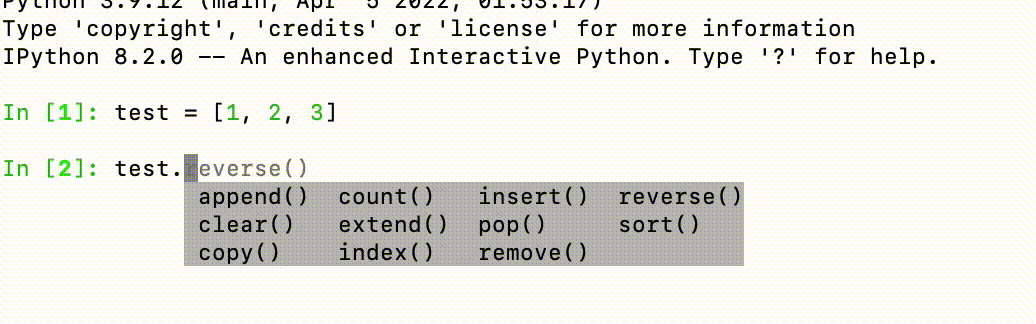
\includegraphics{./assets/tab-complete.png}

\begin{tcolorbox}[enhanced jigsaw, bottomrule=.15mm, arc=.35mm, titlerule=0mm, breakable, coltitle=black, leftrule=.75mm, opacitybacktitle=0.6, colbacktitle=quarto-callout-tip-color!10!white, rightrule=.15mm, bottomtitle=1mm, toptitle=1mm, left=2mm, opacityback=0, toprule=.15mm, title=\textcolor{quarto-callout-tip-color}{\faLightbulb}\hspace{0.5em}{Dunder methods}, colback=white, colframe=quarto-callout-tip-color-frame]

You can list all of an objects properties and methods using
\texttt{dir}:

\begin{Shaded}
\begin{Highlighting}[]
\BuiltInTok{dir}\NormalTok{(my\_list)}
\end{Highlighting}
\end{Shaded}

\begin{verbatim}
['__add__',
 '__class__',
 '__class_getitem__',
 '__contains__',
 '__delattr__',
 '__delitem__',
 '__dir__',
 '__doc__',
 '__eq__',
 '__format__',
 '__ge__',
 '__getattribute__',
 '__getitem__',
 '__gt__',
 '__hash__',
 '__iadd__',
 '__imul__',
 '__init__',
 '__init_subclass__',
 '__iter__',
 '__le__',
 '__len__',
 '__lt__',
 '__mul__',
 '__ne__',
 '__new__',
 '__reduce__',
 '__reduce_ex__',
 '__repr__',
 '__reversed__',
 '__rmul__',
 '__setattr__',
 '__setitem__',
 '__sizeof__',
 '__str__',
 '__subclasshook__',
 'append',
 'clear',
 'copy',
 'count',
 'extend',
 'index',
 'insert',
 'pop',
 'remove',
 'reverse',
 'sort']
\end{verbatim}

Notice that lots of these are methods have a name sandwiched between
double underscores and for this reason are called \emph{dunder methods}
(or \emph{magic methods}, or just \emph{special methods}). This is to
indicate that they are not to be used by you, but by the Python
interpreter to implement certain standard functions that apply to many
different classes of objects. For instance, when you write
\texttt{len(my\_list)} to find the length of \texttt{my\_list} Python is
actually calling the dunder method \texttt{my\_list.\_\_len\_\_} which
does the job of actually finding the length.

\begin{Shaded}
\begin{Highlighting}[]
\NormalTok{my\_list.}\FunctionTok{\_\_len\_\_}\NormalTok{()}
\end{Highlighting}
\end{Shaded}

\begin{verbatim}
4
\end{verbatim}

In this way the same function (\texttt{len} in this case) can operate on
many different objects, an example of what is called
\href{https://en.wikipedia.org/wiki/Polymorphism_(computer_science)}{polymorphism}
in object oriented programming.

\end{tcolorbox}

\hypertarget{arrays}{%
\section{Arrays}\label{arrays}}

The fundamental object in NumPy is the \emph{Array}, which you can think
of as a multidimensional version of a list. Let's start with two
dimensions to demonstrate:

\begin{Shaded}
\begin{Highlighting}[]
\ImportTok{import}\NormalTok{ numpy }\ImportTok{as}\NormalTok{ np}
\NormalTok{my\_array }\OperatorTok{=}\NormalTok{ np.array([[}\DecValTok{1}\NormalTok{, }\DecValTok{2}\NormalTok{, }\DecValTok{3}\NormalTok{], [}\DecValTok{4}\NormalTok{, }\DecValTok{5}\NormalTok{, }\DecValTok{6}\NormalTok{], [}\DecValTok{7}\NormalTok{, }\DecValTok{8}\NormalTok{, }\DecValTok{9}\NormalTok{], [}\DecValTok{10}\NormalTok{, }\DecValTok{11}\NormalTok{, }\DecValTok{12}\NormalTok{]])}
\end{Highlighting}
\end{Shaded}

\begin{Shaded}
\begin{Highlighting}[]
\BuiltInTok{type}\NormalTok{(my\_array)}
\end{Highlighting}
\end{Shaded}

\begin{verbatim}
numpy.ndarray
\end{verbatim}

Arrays can be indexed, similar to lists

\begin{Shaded}
\begin{Highlighting}[]
\BuiltInTok{print}\NormalTok{(my\_array[}\DecValTok{0}\NormalTok{], my\_array[}\DecValTok{1}\NormalTok{], my\_array[}\DecValTok{3}\NormalTok{][}\DecValTok{1}\NormalTok{])}
\end{Highlighting}
\end{Shaded}

\begin{verbatim}
[1 2 3] [4 5 6] 11
\end{verbatim}

but -- different from a ordinary list of lists -- the last one can be
much more pleasantly achieved with the syntax

\begin{Shaded}
\begin{Highlighting}[]
\NormalTok{my\_array[}\DecValTok{3}\NormalTok{,}\DecValTok{1}\NormalTok{]}
\end{Highlighting}
\end{Shaded}

\begin{verbatim}
11
\end{verbatim}

We also have a generalization of the slice syntax

\begin{Shaded}
\begin{Highlighting}[]
\NormalTok{my\_array[}\DecValTok{1}\NormalTok{:, }\DecValTok{1}\NormalTok{:]}
\end{Highlighting}
\end{Shaded}

\begin{verbatim}
array([[ 5,  6],
       [ 8,  9],
       [11, 12]])
\end{verbatim}

Slicing can be mixed with integer indexing

\begin{Shaded}
\begin{Highlighting}[]
\NormalTok{my\_array[}\DecValTok{1}\NormalTok{:, }\DecValTok{1}\NormalTok{]}
\end{Highlighting}
\end{Shaded}

\begin{verbatim}
array([ 5,  8, 11])
\end{verbatim}

NumPy offers all sorts of fancy indexing options for slicing and dicing
your data: see the
\href{https://numpy.org/doc/stable/user/basics.indexing.html}{documentation}
for details.

A fundamental property of an array is its \texttt{shape}:

\begin{Shaded}
\begin{Highlighting}[]
\CommentTok{\# [[1, 2, 3], [4, 5, 6], [7, 8, 9], [10, 11, 12]]}
\NormalTok{my\_array.shape}
\end{Highlighting}
\end{Shaded}

\begin{verbatim}
(4, 3)
\end{verbatim}

The way to read off the shape of an array is as follows. To begin with
you encounter a number of \texttt{{[}} corresponding to the rank of the
array (two in the above example). You then scan over a number of entries
that give the rightmost (innermost) dimension in the shape tuple before
closing \texttt{{]}} (3 here). After a number of 1D arrays
\texttt{{[}...{]}} equal to the next innermost dimension (4 here), we
have another closing \texttt{{]}}, and so on.

It's definitely something that will take a bit of time getting used to!

Notice that slicing does not change the rank of the array

\begin{Shaded}
\begin{Highlighting}[]
\NormalTok{my\_array[}\DecValTok{1}\NormalTok{:, }\DecValTok{1}\NormalTok{:].shape}
\end{Highlighting}
\end{Shaded}

\begin{verbatim}
(3, 2)
\end{verbatim}

but integer indexing does

\begin{Shaded}
\begin{Highlighting}[]
\NormalTok{my\_array[}\DecValTok{1}\NormalTok{:, }\DecValTok{1}\NormalTok{].shape}
\end{Highlighting}
\end{Shaded}

\begin{verbatim}
(3,)
\end{verbatim}

NumPy has lots of methods to create arrays with a given shape and
populated in different ways:

\begin{Shaded}
\begin{Highlighting}[]
\NormalTok{a }\OperatorTok{=}\NormalTok{ np.zeros((}\DecValTok{2}\NormalTok{,}\DecValTok{2}\NormalTok{))}
\BuiltInTok{print}\NormalTok{(a)}

\NormalTok{b }\OperatorTok{=}\NormalTok{ np.ones((}\DecValTok{2}\NormalTok{,}\DecValTok{2}\NormalTok{))}
\BuiltInTok{print}\NormalTok{(b)}

\NormalTok{c }\OperatorTok{=}\NormalTok{ np.full((}\DecValTok{2}\NormalTok{,}\DecValTok{2}\NormalTok{), }\DecValTok{5}\NormalTok{)}
\BuiltInTok{print}\NormalTok{(c)}

\NormalTok{d }\OperatorTok{=}\NormalTok{ np.random.random((}\DecValTok{2}\NormalTok{,}\DecValTok{2}\NormalTok{)) }\CommentTok{\# random numbers uniformly in [0.0, 1.0)}
\BuiltInTok{print}\NormalTok{(d)}
\end{Highlighting}
\end{Shaded}

\begin{verbatim}
[[0. 0.]
 [0. 0.]]
[[1. 1.]
 [1. 1.]]
[[5 5]
 [5 5]]
[[0.06254687 0.06180034]
 [0.55375253 0.67684538]]
\end{verbatim}

There are also lots of methods to change the shape of arrays, for
example

\begin{itemize}
\item
  \href{https://numpy.org/doc/stable/reference/generated/numpy.reshape.html\#numpy-reshape}{numpy.reshape}
  to change the shape of an array.
\item
  \href{https://numpy.org/doc/stable/reference/generated/numpy.expand_dims.html}{numpy.expand\_dims}
  to insert new axes of length one.
\item
  \href{https://numpy.org/doc/stable/reference/generated/numpy.squeeze.html\#numpy.squeeze}{numpy.squeeze}
  (the opposite) to remove new axes of length one.
\end{itemize}

A NumPy array has a \texttt{dtype} property that gives the datatype. If
the array was created from data, this will be inferred

\begin{Shaded}
\begin{Highlighting}[]
\NormalTok{my\_array.dtype}
\end{Highlighting}
\end{Shaded}

\begin{verbatim}
dtype('int64')
\end{verbatim}

Functions that construct arrays also have an optional argument to
specify the datatype

\begin{Shaded}
\begin{Highlighting}[]
\NormalTok{my\_float\_array }\OperatorTok{=}\NormalTok{ np.array([}\DecValTok{1}\NormalTok{,}\DecValTok{2}\NormalTok{,}\DecValTok{3}\NormalTok{], dtype}\OperatorTok{=}\NormalTok{np.float64)}
\NormalTok{my\_float\_array.dtype}
\end{Highlighting}
\end{Shaded}

\begin{verbatim}
dtype('float64')
\end{verbatim}

\hypertarget{mathematical-operations-with-arrays}{%
\section{Mathematical operations with
arrays}\label{mathematical-operations-with-arrays}}

Now here comes the payoff. On lists, multiplication by an integer
concatentates multiple copies

\begin{Shaded}
\begin{Highlighting}[]
\DecValTok{2} \OperatorTok{*}\NormalTok{ [}\DecValTok{1}\NormalTok{, }\DecValTok{2}\NormalTok{, }\DecValTok{3}\NormalTok{]}
\end{Highlighting}
\end{Shaded}

\begin{verbatim}
[1, 2, 3, 1, 2, 3]
\end{verbatim}

which is sometimes useful. But in numerical applications what we really
want is this

\begin{Shaded}
\begin{Highlighting}[]
\DecValTok{2} \OperatorTok{*}\NormalTok{ np.array([}\DecValTok{1}\NormalTok{, }\DecValTok{2}\NormalTok{, }\DecValTok{3}\NormalTok{])}
\end{Highlighting}
\end{Shaded}

\begin{verbatim}
array([2, 4, 6])
\end{verbatim}

This illustrates a general feature of NumPy that \textbf{all
mathematical operations are performed elementwise on arrays!}

\begin{Shaded}
\begin{Highlighting}[]
\BuiltInTok{print}\NormalTok{(np.array([}\DecValTok{1}\NormalTok{, }\DecValTok{2}\NormalTok{, }\DecValTok{3}\NormalTok{]) }\OperatorTok{+}\NormalTok{ np.array([}\DecValTok{4}\NormalTok{, }\DecValTok{5}\NormalTok{, }\DecValTok{6}\NormalTok{]))}
\BuiltInTok{print}\NormalTok{(np.array([}\DecValTok{1}\NormalTok{, }\DecValTok{2}\NormalTok{, }\DecValTok{3}\NormalTok{])}\OperatorTok{**}\DecValTok{2}\NormalTok{)}
\BuiltInTok{print}\NormalTok{(np.sqrt(np.array([}\DecValTok{1}\NormalTok{, }\DecValTok{2}\NormalTok{, }\DecValTok{3}\NormalTok{])))}
\end{Highlighting}
\end{Shaded}

\begin{verbatim}
[5 7 9]
[1 4 9]
[1.         1.41421356 1.73205081]
\end{verbatim}

This avoids the need to write nested loops to perform some operation on
each element of some multidimensional data. Of course, the loops are
still there, it's just that NumPy handles them in highly optimized C
rather than Python. Code which operates in this way -- rather than with
explicit loops -- is often described as \emph{vectorized}, and in
NumPy-speak vectorized functions are called \emph{ufuncs}, short for
\emph{universal functions} (you can
\href{https://numpy.org/doc/stable/reference/ufuncs.html}{write your
own} if you need to). As a basic principle you should \emph{never} use a
Python loop to access your data in NumPy code. Loops may appear at a
high level in stepping through time steps in a simulation, for example.

\hypertarget{broadcasting}{%
\subsection{Broadcasting}\label{broadcasting}}

Vectorization is even more versatile than the above examples might
suggest. \emph{Broadcasting} is a powerful protocol that allows us to
combine arrays of different shapes. Thus we can add a number to an array

\begin{Shaded}
\begin{Highlighting}[]
\NormalTok{np.array([}\DecValTok{1}\NormalTok{, }\DecValTok{2}\NormalTok{, }\DecValTok{3}\NormalTok{]) }\OperatorTok{+} \FloatTok{2.3}
\end{Highlighting}
\end{Shaded}

\begin{verbatim}
array([3.3, 4.3, 5.3])
\end{verbatim}

More generally, elementwise operations can be performed on two arrays of
the same rank if in each dimension the sizes either match or one array
has size 1.

\begin{Shaded}
\begin{Highlighting}[]
\CommentTok{\# These have shape (2, 3) and (1, 3)}
\NormalTok{np.array([[}\DecValTok{1}\NormalTok{, }\DecValTok{2}\NormalTok{, }\DecValTok{3}\NormalTok{], [}\DecValTok{4}\NormalTok{, }\DecValTok{5}\NormalTok{, }\DecValTok{6}\NormalTok{]]) }\OperatorTok{+}\NormalTok{ np.array([[}\DecValTok{4}\NormalTok{, }\DecValTok{3}\NormalTok{, }\DecValTok{2}\NormalTok{]])}
\end{Highlighting}
\end{Shaded}

\begin{verbatim}
array([[5, 5, 5],
       [8, 8, 8]])
\end{verbatim}

In fact, we can simplify this last example

\begin{Shaded}
\begin{Highlighting}[]
\CommentTok{\# These have shape (2, 3) and (3,)}
\NormalTok{np.array([[}\DecValTok{1}\NormalTok{, }\DecValTok{2}\NormalTok{, }\DecValTok{3}\NormalTok{], [}\DecValTok{4}\NormalTok{, }\DecValTok{5}\NormalTok{, }\DecValTok{6}\NormalTok{]]) }\OperatorTok{+}\NormalTok{ np.array([}\DecValTok{4}\NormalTok{, }\DecValTok{3}\NormalTok{, }\DecValTok{2}\NormalTok{])}
\end{Highlighting}
\end{Shaded}

\begin{verbatim}
array([[5, 5, 5],
       [8, 8, 8]])
\end{verbatim}

Broadcasting two arrays follows these rules:

\begin{enumerate}
\def\labelenumi{\arabic{enumi}.}
\item
  If the arrays do not have the same rank, prepend the shape of the
  lower rank array with 1s until both shapes have the same length.
\item
  The two arrays are said to be compatible in a dimension if they have
  the same size in the dimension, or if one of the arrays has size 1 in
  that dimension.
\item
  The arrays can be broadcast together if they are compatible in all
  dimensions. After broadcasting, each array behaves as if it had shape
  equal to the elementwise maximum of shapes of the two input arrays.
\item
  In any dimension where one array had size 1 and the other array had
  size greater than 1, the first array behaves as if it were copied
  along that dimension.
\end{enumerate}

\href{https://numpy.org/doc/stable/user/basics.broadcasting.html}{The
documentation} has more detail.

\hypertarget{example-playing-with-images}{%
\subsection{Example: playing with
images}\label{example-playing-with-images}}

Nice example of a 2D array?

TODO

\hypertarget{plotting-with-matplotlib}{%
\section{Plotting with Matplotlib}\label{plotting-with-matplotlib}}

There are various specialized Python plotting libraries but the
entry-level option is the catchily named
\href{https://matplotlib.org/}{Matplotlib}. The \texttt{pyplot} module
provides a plotting system that is similar to MATLAB (I'm told)

\begin{Shaded}
\begin{Highlighting}[]
\ImportTok{import}\NormalTok{ matplotlib.pyplot }\ImportTok{as}\NormalTok{ plt}
\end{Highlighting}
\end{Shaded}

Here's a simple example of the \texttt{plot} function, used to plot 2D
data

\begin{Shaded}
\begin{Highlighting}[]
\CommentTok{\# Compute the x and y coordinates for points on a sine curve}
\NormalTok{x }\OperatorTok{=}\NormalTok{ np.arange(}\DecValTok{0}\NormalTok{, }\DecValTok{3} \OperatorTok{*}\NormalTok{ np.pi, }\FloatTok{0.1}\NormalTok{)}
\NormalTok{y }\OperatorTok{=}\NormalTok{ np.sin(x)}

\CommentTok{\# Plot the points using matplotlib}
\NormalTok{plt.plot(x, y)}
\NormalTok{plt.show()}
\end{Highlighting}
\end{Shaded}

\begin{figure}[H]

{\centering 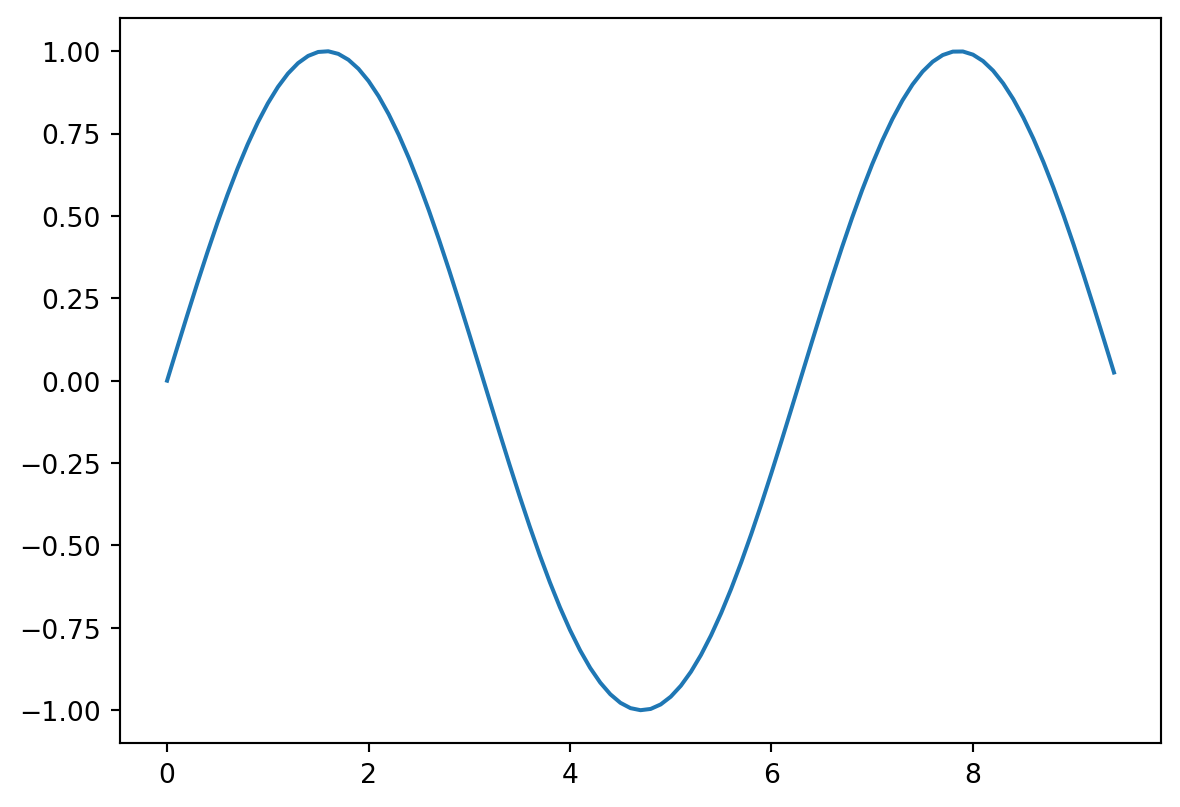
\includegraphics{./numpy_files/figure-pdf/cell-25-output-1.pdf}

}

\end{figure}

\textbf{Note}: you must call plt.show() to make graphics appear. Here's
a fancier example with some labelling

\begin{Shaded}
\begin{Highlighting}[]
\CommentTok{\# Compute the x and y coordinates for points on sine and cosine curves}
\NormalTok{x }\OperatorTok{=}\NormalTok{ np.arange(}\DecValTok{0}\NormalTok{, }\DecValTok{3} \OperatorTok{*}\NormalTok{ np.pi, }\FloatTok{0.1}\NormalTok{)}
\NormalTok{y\_sin }\OperatorTok{=}\NormalTok{ np.sin(x)}
\NormalTok{y\_cos }\OperatorTok{=}\NormalTok{ np.cos(x)}

\CommentTok{\# Plot the points using matplotlib}
\NormalTok{plt.plot(x, y\_sin)}
\NormalTok{plt.plot(x, y\_cos)}
\NormalTok{plt.xlabel(}\StringTok{\textquotesingle{}x axis label\textquotesingle{}}\NormalTok{)}
\NormalTok{plt.ylabel(}\StringTok{\textquotesingle{}y axis label\textquotesingle{}}\NormalTok{)}
\NormalTok{plt.title(}\StringTok{\textquotesingle{}Sine and Cosine\textquotesingle{}}\NormalTok{)}
\NormalTok{plt.legend([}\StringTok{\textquotesingle{}Sine\textquotesingle{}}\NormalTok{, }\StringTok{\textquotesingle{}Cosine\textquotesingle{}}\NormalTok{])}
\NormalTok{plt.show()}
\end{Highlighting}
\end{Shaded}

\begin{figure}[H]

{\centering 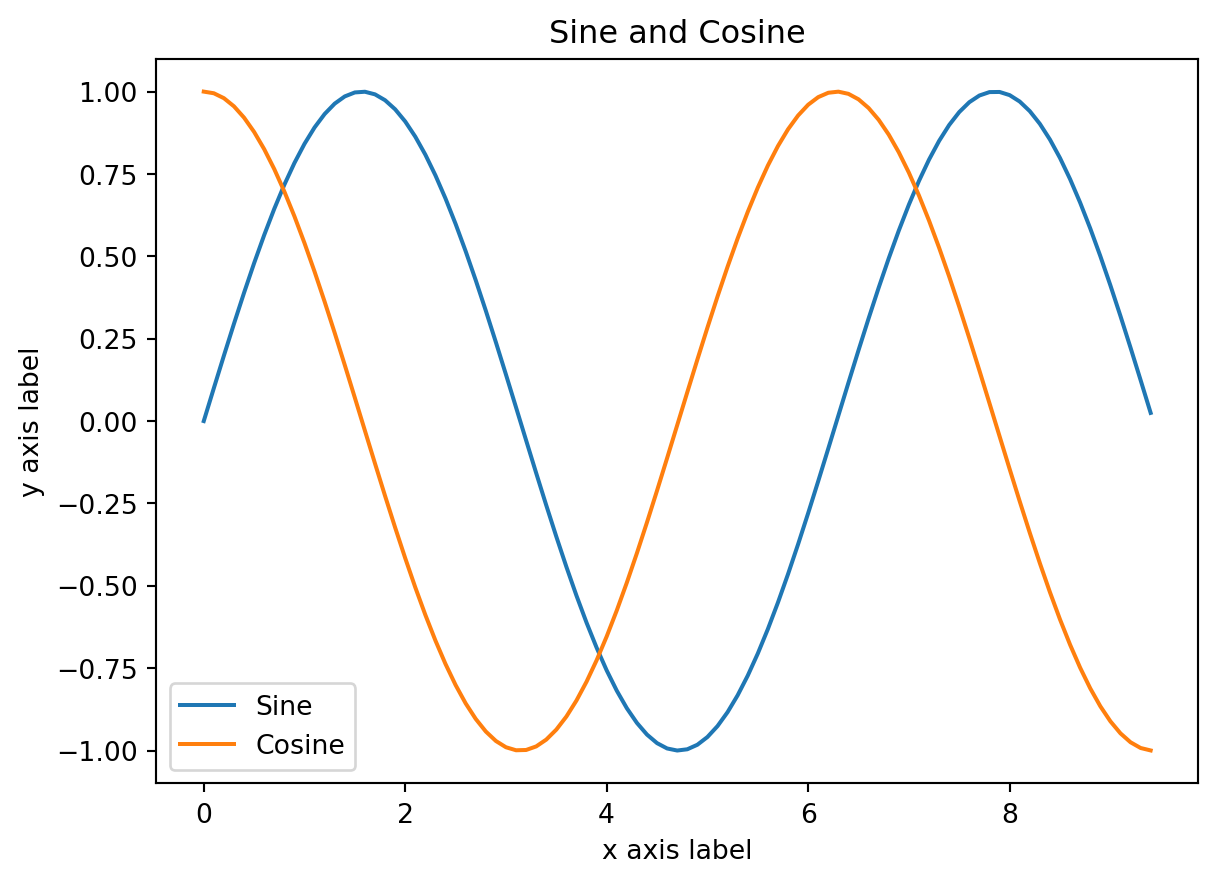
\includegraphics{./numpy_files/figure-pdf/cell-26-output-1.pdf}

}

\end{figure}

Often you'll want to make several related plots and present them
together, which can be achieved using the \texttt{subplot} function

\begin{Shaded}
\begin{Highlighting}[]
\ImportTok{import}\NormalTok{ numpy }\ImportTok{as}\NormalTok{ np}
\ImportTok{import}\NormalTok{ matplotlib.pyplot }\ImportTok{as}\NormalTok{ plt}

\CommentTok{\# Compute the x and y coordinates for points on sine and cosine curves}
\NormalTok{x }\OperatorTok{=}\NormalTok{ np.arange(}\DecValTok{0}\NormalTok{, }\DecValTok{3} \OperatorTok{*}\NormalTok{ np.pi, }\FloatTok{0.1}\NormalTok{)}
\NormalTok{y\_sin }\OperatorTok{=}\NormalTok{ np.sin(x)}
\NormalTok{y\_cos }\OperatorTok{=}\NormalTok{ np.cos(x)}

\CommentTok{\# Set up a subplot grid that has height 2 and width 1,}
\CommentTok{\# and set the first such subplot as active.}
\NormalTok{plt.subplot(}\DecValTok{2}\NormalTok{, }\DecValTok{1}\NormalTok{, }\DecValTok{1}\NormalTok{)}

\CommentTok{\# Make the first plot}
\NormalTok{plt.plot(x, y\_sin)}
\NormalTok{plt.title(}\StringTok{\textquotesingle{}Sine\textquotesingle{}}\NormalTok{)}

\CommentTok{\# Set the second subplot as active, and make the second plot.}
\NormalTok{plt.subplot(}\DecValTok{2}\NormalTok{, }\DecValTok{1}\NormalTok{, }\DecValTok{2}\NormalTok{)}
\NormalTok{plt.plot(x, y\_cos)}
\NormalTok{plt.title(}\StringTok{\textquotesingle{}Cosine\textquotesingle{}}\NormalTok{)}

\CommentTok{\# Show the figure.}
\NormalTok{plt.show()}
\end{Highlighting}
\end{Shaded}

\begin{figure}[H]

{\centering 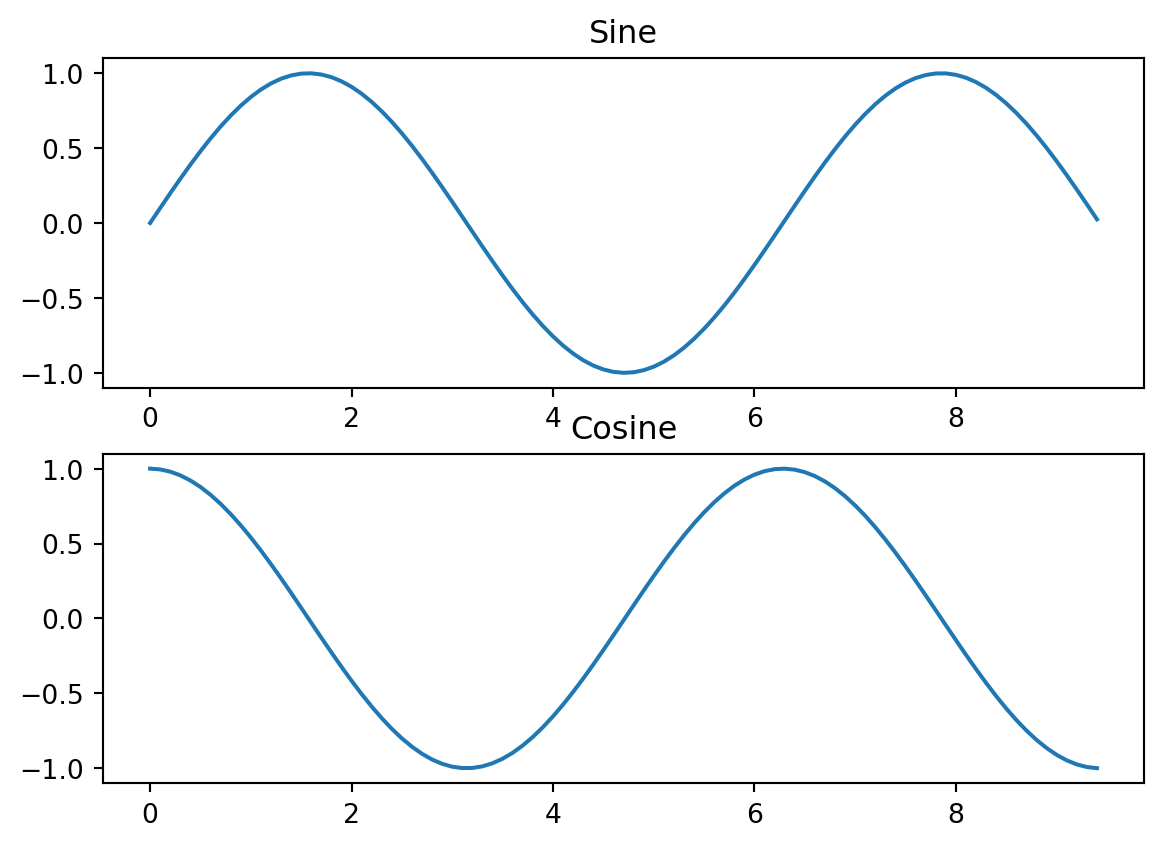
\includegraphics{./numpy_files/figure-pdf/cell-27-output-1.pdf}

}

\end{figure}

\hypertarget{saving-and-loading-data}{%
\section{Saving and loading data}\label{saving-and-loading-data}}

In the course of your work you are likely to produce, as well as consume
lots of data. While it's good practice to keep notebooks capable of
reproducing any of your analyses, this could be time consuming and
resource heavy for larger computations. Thus at some point you'll
probably want to save and load data. For example, after saving the data
of a large scale simulation you'd like to load it and perform some
analysis.

NumPy comes with its own
\href{https://numpy.org/doc/stable/reference/generated/numpy.save.html}{save}
and
\href{https://numpy.org/doc/stable/reference/generated/numpy.load.html}{load}
functions and associated binary format \texttt{.npy}. The benefit of
using these is that after loading you get back a NumPy array ready to be
used.

A related function
\href{https://numpy.org/doc/stable/reference/generated/numpy.savez.html}{savez}
allows several arrays to be saved and then loaded as a dictionary-like
object.

\bookmarksetup{startatroot}

\hypertarget{floating-point-and-all-that}{%
\chapter{Floating point and all
that}\label{floating-point-and-all-that}}

Since physics is all about numbers we had better develop some
understanding of how computers represent them, and the limitations of
this representation. Hopefully this example is sufficiently motivating:

\begin{Shaded}
\begin{Highlighting}[]
\FloatTok{0.1}  \OperatorTok{+} \FloatTok{0.2} \OperatorTok{==} \FloatTok{0.3}
\end{Highlighting}
\end{Shaded}

\begin{verbatim}
False
\end{verbatim}

Ah\ldots{}

\hypertarget{integers}{%
\section{Integers}\label{integers}}

Let's begin with something simpler

\begin{Shaded}
\begin{Highlighting}[]
\DecValTok{1} \OperatorTok{+} \DecValTok{1} \OperatorTok{==} \DecValTok{2}
\end{Highlighting}
\end{Shaded}

\begin{verbatim}
True
\end{verbatim}

which is a bit more reassuring. Integers can be represented in binary

\begin{Shaded}
\begin{Highlighting}[]
\DecValTok{3} \OperatorTok{==} \BaseNTok{0b11}
\end{Highlighting}
\end{Shaded}

\begin{verbatim}
True
\end{verbatim}

or octal or hexadecimal (with a prefix \texttt{0o} or \texttt{0h}). You
can get the binary string representing an integer using the \texttt{bin}
function

\begin{Shaded}
\begin{Highlighting}[]
\BuiltInTok{bin}\NormalTok{(}\OperatorTok{{-}}\DecValTok{2}\NormalTok{)}
\end{Highlighting}
\end{Shaded}

\begin{verbatim}
'-0b10'
\end{verbatim}

Python allows for arbitrarily large integers, so there is no possibility
of overflow or rounding error

\begin{Shaded}
\begin{Highlighting}[]
\DecValTok{2}\OperatorTok{**}\DecValTok{100}
\end{Highlighting}
\end{Shaded}

\begin{verbatim}
1267650600228229401496703205376
\end{verbatim}

The only limitation is the memory required to store it.

Numpy integers are a different story

\begin{Shaded}
\begin{Highlighting}[]
\ImportTok{import}\NormalTok{ numpy }\ImportTok{as}\NormalTok{ np}
\NormalTok{np.int64(}\DecValTok{2}\OperatorTok{**}\DecValTok{100}\NormalTok{)}
\end{Highlighting}
\end{Shaded}

\begin{verbatim}
OverflowError: Python int too large to convert to C long
\end{verbatim}

Since NumPy is using C the types have to play nicely. The range of
integers that can be represented with 32 bit \texttt{numpy.int32}s is
\(\approx\pm 2^{31} \approx \pm 2.1 × 10^9\) (one bit is for the sign)
and 64 bit \texttt{numpy.int64}s is
\(\approx\pm 2^{63} \approx \pm 9.2 × 10^{18}\). Apart from the risk of
overflow when working NumPy's integers there are not other gotchas to
worry about.

\hypertarget{floating-point-numbers}{%
\section{Floating point numbers}\label{floating-point-numbers}}

The reason why \(0.1 + 0.2 \neq 0.3\) in Python is that specifying a
real number exactly would involve an infinite number of bits, so that
any finite representation is necessarily approximate.

The representation computers use for the reals is called
\href{https://en.wikipedia.org/wiki/Floating-point_arithmetic}{floating
point arithmetic}. It is essentially a form of scientific notation, in
which a \href{https://en.wikipedia.org/wiki/Significand}{significand}
(it contains the significant figures) is multiplied by an
\emph{exponent}. The name \emph{floating point} reflects the fact that
the number of digits after the decimal point is not fixed (I'm using the
base ten terms for convenience)

This representation requires the choice of a base, and Python's floating
point numbers use binary. Numbers with finite binary representations
therefore behave nicely

\begin{Shaded}
\begin{Highlighting}[]
\FloatTok{0.125} \OperatorTok{+} \FloatTok{0.25} \OperatorTok{==} \FloatTok{0.375}
\end{Highlighting}
\end{Shaded}

\begin{verbatim}
True
\end{verbatim}

For decimal numbers to be represented exactly we'd have to use base ten.
This can be achieved with the \texttt{decimal} module. Our \(0.1+0.2\)
example then works as expected

\begin{Shaded}
\begin{Highlighting}[]
\ImportTok{from}\NormalTok{ decimal }\ImportTok{import} \OperatorTok{*}
\NormalTok{Decimal(}\StringTok{\textquotesingle{}0.1\textquotesingle{}}\NormalTok{) }\OperatorTok{+}\NormalTok{ Decimal(}\StringTok{\textquotesingle{}0.2\textquotesingle{}}\NormalTok{)}
\end{Highlighting}
\end{Shaded}

\begin{verbatim}
Decimal('0.3')
\end{verbatim}

Since there is nothing to single out the decimal representation in
physics (as opposed to, say, finance) we won't have any need for it.

A specification for floating point numbers must give

\begin{enumerate}
\def\labelenumi{\arabic{enumi}.}
\tightlist
\item
  A base (or \emph{radix}) \(b\)
\item
  A precision \(p\), the number of digits in the significand \(c\). Thus
  \(0\leq c \leq b^{p}-1\).
\item
  A range of exponents \(q\) specifed by \(\text{emin}\) and
  \(\text{emax}\) with \(\text{emin}\leq q+p-1 \leq \text{emax}\).
\end{enumerate}

Including one bit \(s\) for the overall sign, a number then has the form
\((-1)^s\times c \times b^q\). The smallest positive nonzero number that
can be represented is therefore \(b^{1 + \text{emin} - p}\)
(corresponding to the smallest value of the exponent) and the largest is
\(b^{1 + \text{emax}} - 1\).

The above representation isn't unique: for some numbers you could make
the significand smaller and the exponent bigger. A unique representation
is fixed by choosing the exponent to be as small as possible.

Representing numbers smaller than \(b^{\text{emin}}\) involves a loss of
precision, as the number of digits in the significand falls below \(p\)
and the exponent has taken its minimum value . These are called
\href{https://en.wikipedia.org/wiki/Subnormal_number}{subnormal
numbers}. For binary floats, if we stick with the normal numbers and a
\(p\)-bit significand the leading bit will be 1 and so can be dropped
from the representation, which then only requires \(p-1\) bits.

The specification for the floating point numbers used by Python (and
many other languages) is contained in the IEEE Standard for Floating
Point Arithmetic \href{https://en.wikipedia.org/wiki/IEEE_754}{IEEE
754}. The default Python \texttt{float} uses the 64 bit \emph{binary64}
representation (often called \emph{double precision}). Here's how those
64 bits are used

\begin{itemize}
\tightlist
\item
  \(p=53\) for the significand, encoded in 52 bits
\item
  11 bits for the exponent
\item
  1 bit for the sign
\end{itemize}

Another common representation is the 32 bit \emph{binary32}
(\emph{single precision}) with

\begin{itemize}
\tightlist
\item
  \(p=24\) for the significand, encoded in 23 bits
\item
  8 bits for the exponent
\item
  1 bit for the sign
\end{itemize}

\hypertarget{sec-fp-numpy}{%
\subsection{Floating point numbers in NumPy}\label{sec-fp-numpy}}

If this all a bit theoretical you can just get NumPy's
\href{https://numpy.org/doc/stable/reference/generated/numpy.finfo.html}{finfo}
function to tell all about the
\href{https://en.wikipedia.org/wiki/Machine_epsilon}{machine precision}

\begin{Shaded}
\begin{Highlighting}[]
\NormalTok{np.finfo(np.float64)}
\end{Highlighting}
\end{Shaded}

\begin{verbatim}
finfo(resolution=1e-15, min=-1.7976931348623157e+308, max=1.7976931348623157e+308, dtype=float64)
\end{verbatim}

Note that \(2^{-52}=2.22\times 10^{-16}\) which accounts for the value
\(10^{-15}\) of the resolution. This can be checked by finding when a
number is close enough to treated as 1.0.

\begin{Shaded}
\begin{Highlighting}[]
\NormalTok{x}\OperatorTok{=}\FloatTok{1.0}
\ControlFlowTok{while} \FloatTok{1.0} \OperatorTok{+}\NormalTok{ x }\OperatorTok{!=} \FloatTok{1.0}\NormalTok{:}
\NormalTok{    x }\OperatorTok{/=} \FloatTok{1.01} 
\BuiltInTok{print}\NormalTok{(x)}
\end{Highlighting}
\end{Shaded}

\begin{verbatim}
1.099427563084686e-16
\end{verbatim}

For binary32 we have a resolution of \(10^{-6}\).

\begin{Shaded}
\begin{Highlighting}[]
\NormalTok{np.finfo(np.float32)}
\end{Highlighting}
\end{Shaded}

\begin{verbatim}
finfo(resolution=1e-06, min=-3.4028235e+38, max=3.4028235e+38, dtype=float32)
\end{verbatim}

One lesson from this is that taking small differences between numbers is
a potential source of rounding error, as in this somewhat mean exam
question

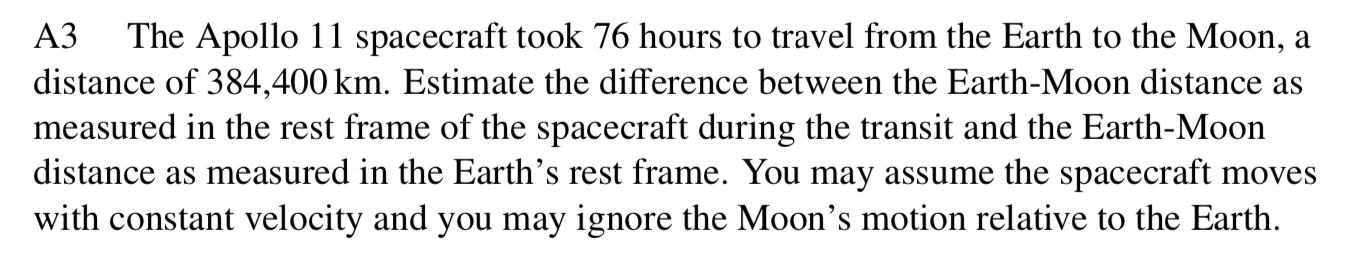
\includegraphics{./assets/ia-question.png}

\begin{tcolorbox}[enhanced jigsaw, bottomrule=.15mm, arc=.35mm, titlerule=0mm, breakable, coltitle=black, leftrule=.75mm, opacitybacktitle=0.6, colbacktitle=quarto-callout-tip-color!10!white, rightrule=.15mm, bottomtitle=1mm, toptitle=1mm, left=2mm, opacityback=0, toprule=.15mm, title=\textcolor{quarto-callout-tip-color}{\faLightbulb}\hspace{0.5em}{Solution}, colback=white, colframe=quarto-callout-tip-color-frame]

Solution: \(x-x'=x(1-\gamma^{-1})\sim x\beta^2/2\sim 4.2\text{mm}\).

\begin{Shaded}
\begin{Highlighting}[]
\ImportTok{import}\NormalTok{ numpy }\ImportTok{as}\NormalTok{ np}
\ImportTok{from}\NormalTok{ scipy.constants }\ImportTok{import}\NormalTok{ c}
\NormalTok{beta }\OperatorTok{=} \FloatTok{384400e3} \OperatorTok{/}\NormalTok{ (}\DecValTok{76} \OperatorTok{*} \DecValTok{3600}\NormalTok{) }\OperatorTok{/}\NormalTok{ c}
\NormalTok{gamma }\OperatorTok{=} \DecValTok{1}\OperatorTok{/}\NormalTok{np.sqrt(}\DecValTok{1} \OperatorTok{{-}}\NormalTok{ beta}\OperatorTok{**}\DecValTok{2}\NormalTok{)}
\BuiltInTok{print}\NormalTok{(}\DecValTok{1} \OperatorTok{{-}}\NormalTok{ np.float32(}\DecValTok{1}\OperatorTok{/}\NormalTok{gamma), }\DecValTok{1} \OperatorTok{{-}}\NormalTok{ np.float64(}\DecValTok{1}\OperatorTok{/}\NormalTok{gamma))}
\end{Highlighting}
\end{Shaded}

\begin{verbatim}
0.0 1.0981660025777273e-11
\end{verbatim}

\end{tcolorbox}

\hypertarget{the-dreaded-nan}{%
\subsection{The dreaded NaN}\label{the-dreaded-nan}}

As well as a floating point system, IEEE 754 defines Infinity and NaN
(Not a Number)

\begin{Shaded}
\begin{Highlighting}[]
\NormalTok{np.array([}\DecValTok{1}\NormalTok{, }\OperatorTok{{-}}\DecValTok{1}\NormalTok{, }\DecValTok{0}\NormalTok{]) }\OperatorTok{/} \DecValTok{0}
\end{Highlighting}
\end{Shaded}

\begin{verbatim}
/var/folders/xs/y8sn45v943s2_62flnxw0p940000gn/T/ipykernel_33246/2604490398.py:1: RuntimeWarning:

divide by zero encountered in true_divide

/var/folders/xs/y8sn45v943s2_62flnxw0p940000gn/T/ipykernel_33246/2604490398.py:1: RuntimeWarning:

invalid value encountered in true_divide
\end{verbatim}

\begin{verbatim}
array([ inf, -inf,  nan])
\end{verbatim}

They behave as you might guess

\begin{Shaded}
\begin{Highlighting}[]
\DecValTok{2} \OperatorTok{*}\NormalTok{ np.inf, }\DecValTok{0} \OperatorTok{*}\NormalTok{ np.inf, np.inf }\OperatorTok{\textgreater{}}\NormalTok{ np.nan}
\end{Highlighting}
\end{Shaded}

\begin{verbatim}
(inf, nan, False)
\end{verbatim}

NaNs propagate through subsequent operations

\begin{Shaded}
\begin{Highlighting}[]
\DecValTok{2} \OperatorTok{*}\NormalTok{ np.nan}
\end{Highlighting}
\end{Shaded}

\begin{verbatim}
nan
\end{verbatim}

which means that if you get a NaN somewhere in your calculation, you'll
probably end up seeing it somewhere in the output (which is the idea).

\bookmarksetup{startatroot}

\hypertarget{solving-differential-equations-with-scipy}{%
\chapter{Solving differential equations with
SciPy}\label{solving-differential-equations-with-scipy}}

\begin{quote}
Newton's fundamental discovery, the one which he considered necessary to
keep secret and published only in the form of an anagram, consists of
the following: \emph{Data aequatione quotcunque fluentes quantitates
involvente, fluxiones invenire; et vice versa}. In contemporary
mathematical language, this means: ``It is useful to solve differential
equations''.

Vladimir Arnold, \emph{Geometrical Methods in the Theory of Ordinary
Differential Equations}
\end{quote}

While Arnold (and Newton) are of course right the problem is that
solving differential equations is \emph{not possible in general}. Even
the simplest example of a first order ordinary differential equation
(ODE) in a single variable

\begin{equation}\protect\hypertarget{eq-ode}{}{
\frac{dx}{dt} = f(x, t)
}\label{eq-ode}\end{equation}

cannot be solved for general \(f(x,t)\) \footnote{Sticking with integers}.
Of course, formulating a physical (or whatever) system in terms of
differential equations represents a nontrivial step on the road to
understanding it, but a lot remains to be done.

Numerical analysis of differential equations is a colossal topic in
applied maths and we are barely going to scratch the surface. The
important thing is to be able to access existing solvers (and implement
your own if necessary) and crucially to \emph{understand their
limitations}.

\hypertarget{eulers-method}{%
\section{Euler's method}\label{eulers-method}}

The basic idea behind all ODE solvers is to introduce a discretization
of the equation and its solution \(x_j\equiv x(t_j)\) at time points
\(t_j = hj\) for some step size \(h\) and \(j=0, 1, \ldots\). The very
simplest approach is called
\href{https://en.wikipedia.org/wiki/Euler_method}{Euler's method}
\footnote{I've borrowed this example from
  \href{https://github.com/CambridgeEngineering/PartIA-Computing-Michaelmas/blob/main/11\%20Complexity.ipynb}{Garth
  Wells' course}} and approximates the derivative on the right hand side
of Equation~\ref{eq-ode} as

\begin{equation}\protect\hypertarget{eq-fwd}{}{
\frac{dx}{dt}\Bigg|_{t=t_j} \approx \frac{x_{j+1} - x_j}{h}.
}\label{eq-fwd}\end{equation}

Rearranging the ODE then gives the update rule

\begin{equation}\protect\hypertarget{eq-euler-update}{}{
x_{j+1} = x_j + hf(x_j, t_j).
}\label{eq-euler-update}\end{equation}

Once an \emph{initial condition} \(x_0\) is specified, subsequent values
can be obtained by iteration.

Notice that Equation~\ref{eq-fwd} involved a
\href{https://en.wikipedia.org/wiki/Finite_difference}{forward finite
difference}: the derivative at time \(t_j\) was approximated in terms of
\(x_j\) and \(x_{j+1}\) (i.e.~one step \emph{forward} in time). Why do
this? So that the update rule Equation~\ref{eq-euler-update} is an
\emph{explicit} formula for \(x_{j+1}\) in terms of \(x_j\). This is
called an \emph{explicit method}. If we had used the backward derivative
we would end up with
\href{https://en.wikipedia.org/wiki/Backward_Euler_method}{backward
Euler method}
\begin{equation}\protect\hypertarget{eq-backward-euler-update}{}{
x_{j+1} = x_j + hf(x_{j+1}, t_{j+1})
}\label{eq-backward-euler-update}\end{equation}

which is \emph{implicit}. This means that the update requires an
additional step to numerically solve for \(x_{j+1}\). Although this is
more costly, there are benefits to the backward method associated with
stability.

\hypertarget{truncation-error}{%
\subsection{Truncation error}\label{truncation-error}}

In making the approximation Equation~\ref{eq-fwd} we make an \(O(h^2)\)
\emph{local truncation error}. To integrate for a fixed time the number
of steps required is proportional to \(h^{-1}\), which means that the
worst case error at fixed time (the \emph{global truncation error}) is
\(O(h)\). For this reason Euler's method is called \emph{first order}.
More sophisticated methods are typically higher order: the SciPy
function
\href{https://docs.scipy.org/doc/scipy/reference/generated/scipy.integrate.solve_ivp.html\#r179348322575-1}{scipy.integrate.solve\_ivp}
uses a fifth order method by default.

TODO discuss midpoint method?

\hypertarget{rounding-error}{%
\subsection{Rounding error}\label{rounding-error}}

If you had unlimited computer time you might think you could make the
step size \(h\) ever smaller in order to make the updates more accurate.
This ignores the machine precision \(\epsilon\), discussed in
Section~\ref{sec-fp-numpy}. The rounding error is roughly
\(\epsilon x_j\), and if the \(N\propto h^{-1}\) errors in successive
steps can be treated as independent random variables, the relative total
rounding error will be
\(\propto \sqrt{N}\epsilon=\frac{\epsilon}{\sqrt{h}}\) and will dominate
for \(h\) small.

\hypertarget{stability}{%
\subsection{Stability}\label{stability}}

Apart from the relatively low accuracy that comes from using a first
order method, the Euler method may additionally be unstable, depending
on the equation. This can be demonstrated for the linear equation

\[
\frac{dx}{dt} = kx
\]

\begin{Shaded}
\begin{Highlighting}[]
\ImportTok{import}\NormalTok{ numpy }\ImportTok{as}\NormalTok{ np}
\ImportTok{import}\NormalTok{ matplotlib.pyplot }\ImportTok{as}\NormalTok{ plt}

\KeywordTok{def}\NormalTok{ euler(h, t\_max, k}\OperatorTok{=}\DecValTok{1}\NormalTok{):}
    \CommentTok{"""}
\CommentTok{    Solve the equation x\textquotesingle{} = k x, with x(0) = 1 using}
\CommentTok{    the Euler method. }

\CommentTok{    Integrate from t=0 to t=t\_max using stepsize h for}
\CommentTok{    num\_steps = t\_max / h.}
\CommentTok{    }
\CommentTok{    Returns two arrays of length num\_steps: t, the time coordinate, and x\_0, the position.}
\CommentTok{    """}
\NormalTok{    num\_steps }\OperatorTok{=} \BuiltInTok{int}\NormalTok{(t\_max }\OperatorTok{/}\NormalTok{ h)}
    \CommentTok{\# Allocate return arrays}
\NormalTok{    x }\OperatorTok{=}\NormalTok{ np.zeros(num\_steps, dtype}\OperatorTok{=}\NormalTok{np.float32)}
\NormalTok{    t }\OperatorTok{=}\NormalTok{ np.zeros(num\_steps, dtype}\OperatorTok{=}\NormalTok{np.float32)}
\NormalTok{    x[}\DecValTok{0}\NormalTok{] }\OperatorTok{=} \FloatTok{1.0}  \CommentTok{\# Initial condition}
    \ControlFlowTok{for}\NormalTok{ i }\KeywordTok{in} \BuiltInTok{range}\NormalTok{(num\_steps }\OperatorTok{{-}} \DecValTok{1}\NormalTok{):}
\NormalTok{        x[i}\OperatorTok{+}\DecValTok{1}\NormalTok{] }\OperatorTok{=}\NormalTok{ x[i] }\OperatorTok{+}\NormalTok{ k }\OperatorTok{*}\NormalTok{ x[i] }\OperatorTok{*}\NormalTok{ h}
\NormalTok{        t[i}\OperatorTok{+}\DecValTok{1}\NormalTok{] }\OperatorTok{=}\NormalTok{ t[i] }\OperatorTok{+}\NormalTok{ h  }\CommentTok{\# Time step}
    \ControlFlowTok{return}\NormalTok{ t, x}

\NormalTok{k }\OperatorTok{=} \OperatorTok{{-}}\FloatTok{2.3}
\NormalTok{t\_max }\OperatorTok{=} \DecValTok{5}
\NormalTok{t, x }\OperatorTok{=}\NormalTok{ euler(}\DecValTok{1}\NormalTok{, t\_max, k)}
\NormalTok{plt.plot(t, x, label}\OperatorTok{=}\StringTok{"h=1 Euler"}\NormalTok{)}
\NormalTok{t, x }\OperatorTok{=}\NormalTok{ euler(}\FloatTok{0.7}\NormalTok{, t\_max, k)}
\NormalTok{plt.plot(t, x, label}\OperatorTok{=}\StringTok{"h=0.7 Euler"}\NormalTok{)}
\NormalTok{t }\OperatorTok{=}\NormalTok{ np.linspace(}\DecValTok{0}\NormalTok{, t\_max, }\DecValTok{100}\NormalTok{)}
\NormalTok{plt.plot(t, np.exp(k }\OperatorTok{*}\NormalTok{ t), label}\OperatorTok{=}\StringTok{"exact solution"}\NormalTok{)}
\NormalTok{plt.title(}\StringTok{"k={-}2.3"}\NormalTok{)}
\NormalTok{plt.legend()}
\NormalTok{plt.show()}
\end{Highlighting}
\end{Shaded}

\begin{figure}[H]

{\centering \includegraphics{./ode_files/figure-pdf/cell-2-output-1.pdf}

}

\end{figure}

For a linear equation the Euler update Equation~\ref{eq-euler-update} is
a simple rescaling

\[
x_{j+1} = x_j(1 + hk)
\]

so the region of stability is \(|1 + hk|\leq 1\). You can check that the
backward Euler method Equation~\ref{eq-backward-euler-update} eliminates
the instability for \(k<0\).

\hypertarget{using-scipy}{%
\section{Using SciPy}\label{using-scipy}}

Coming up with integration schemes is best left to the professionals.
Your first port of call for solving ODEs in Python should probably be
the
\href{https://docs.scipy.org/doc/scipy/tutorial/integrate.html}{integrate}
module of the \href{https://scipy.org/}{SciPy} scientific computing
library. The function
\href{https://docs.scipy.org/doc/scipy/reference/generated/scipy.integrate.solve_ivp.html\#r179348322575-1}{scipy.integrate.solve\_ivp}
provides a versatile API.

One important thing to understand is that all these integration schemes
apply to systems of \emph{first order} differential equations. Higher
order equations can always be presented as a first order system, at the
expense of introducing more equations. For example, in physics we are
often concerned with Newton's equation

\[
m\frac{d^2 \mathbf{x}}{dt^2} = \mathbf{f}(\mathbf{x},t),
\]

which is three second order equations. We turn this into a first order
system by introducing the velocity \(\mathbf{v}=\dot{\mathbf{x}}\),
giving the six equations

\[
\begin{align}
\frac{d\mathbf{x}}{dt} &= \mathbf{v}\\
m\frac{d \mathbf{v}}{dt} &= \mathbf{f}(\mathbf{x},t).
\end{align}
\]

As a simple example, let's consider the pendulum equation

\[
\ddot \theta = -\sin\theta
\]

which can be cast as

\[
\begin{align}
\dot\theta &= l\\
\dot l &= -\sin\theta
\end{align}
\]

Solving the equation using SciPy just requires us to define a function
giving the right hand side of these equations

\begin{Shaded}
\begin{Highlighting}[]
\KeywordTok{def}\NormalTok{ pendulum(t, y): }\ControlFlowTok{return}\NormalTok{ [y[}\DecValTok{1}\NormalTok{], }\OperatorTok{{-}}\NormalTok{np.sin(y[}\DecValTok{0}\NormalTok{])]}
\CommentTok{\# The pendulum equation: y[0] is theta and y[1] is l}
\end{Highlighting}
\end{Shaded}

and then calling \texttt{solve\_ivp}

\begin{Shaded}
\begin{Highlighting}[]
\ImportTok{from}\NormalTok{ scipy.integrate }\ImportTok{import}\NormalTok{ solve\_ivp}
\ImportTok{import}\NormalTok{ matplotlib.pyplot }\ImportTok{as}\NormalTok{ plt}

\NormalTok{t\_max }\OperatorTok{=} \DecValTok{1000}
\NormalTok{pendulum\_motion }\OperatorTok{=}\NormalTok{ solve\_ivp(pendulum, [}\DecValTok{0}\NormalTok{, t\_max], [}\DecValTok{2}\NormalTok{, }\DecValTok{0}\NormalTok{], dense\_output}\OperatorTok{=}\VariableTok{True}\NormalTok{)}
\end{Highlighting}
\end{Shaded}

The option \texttt{dense\_output=True} is used to specify that a
continuous solution should be found. What this means in practice is that
the returned object \texttt{pendulum\_motion} has a \texttt{sol}
property that is an instance of
\href{https://docs.scipy.org/doc/scipy/reference/generated/scipy.integrate.OdeSolution.html\#scipy.integrate.OdeSolution}{OdeSolution}.
\texttt{sol(t)} returns the computed solution at \(t\) (this involves
interpolation). We can use this to plot the pendulum's trajectory in the
\(\theta- l\) \href{https://en.wikipedia.org/wiki/Phase_plane}{phase
plane}, along with the contours of the conserved energy function

\[
E(\theta, l) = \frac{1}{2}l^2 - \cos\theta
\]

\begin{Shaded}
\begin{Highlighting}[]
\NormalTok{fig, ax }\OperatorTok{=}\NormalTok{ plt.subplots()}

\NormalTok{theta }\OperatorTok{=}\NormalTok{ np.linspace(}\OperatorTok{{-}}\FloatTok{1.1} \OperatorTok{*}\NormalTok{ np.pi, }\FloatTok{1.1} \OperatorTok{*}\NormalTok{ np.pi, }\DecValTok{60}\NormalTok{)}
\NormalTok{l }\OperatorTok{=}\NormalTok{ np.linspace(}\OperatorTok{{-}}\DecValTok{2}\NormalTok{, }\DecValTok{2}\NormalTok{, }\DecValTok{60}\NormalTok{)}
\NormalTok{E }\OperatorTok{=} \OperatorTok{{-}}\NormalTok{np.cos(theta[np.newaxis,:]) }\OperatorTok{+}\NormalTok{ (l[:,np.newaxis])}\OperatorTok{**}\DecValTok{2} \OperatorTok{/} \DecValTok{2}
\CommentTok{\# Note the use of broadcasting to obtain the energy as a function of the phase space coordinates}

\NormalTok{xx, yy }\OperatorTok{=}\NormalTok{ np.meshgrid(theta, l)}

\NormalTok{ax.contourf(xx, yy, E, cmap}\OperatorTok{=}\StringTok{\textquotesingle{}Reds\textquotesingle{}}\NormalTok{)}
\NormalTok{t }\OperatorTok{=}\NormalTok{ np.linspace(}\DecValTok{0}\NormalTok{, t\_max, }\DecValTok{10000}\NormalTok{)}
\NormalTok{ax.plot(}\OperatorTok{*}\NormalTok{pendulum\_motion.sol(t))}
\NormalTok{plt.xlabel(}\VerbatimStringTok{r\textquotesingle{}$\textbackslash{}theta$\textquotesingle{}}\NormalTok{)}
\NormalTok{plt.ylabel(}\VerbatimStringTok{r\textquotesingle{}$l$\textquotesingle{}}\NormalTok{)}
\NormalTok{plt.show()}
\end{Highlighting}
\end{Shaded}

\begin{figure}[H]

{\centering 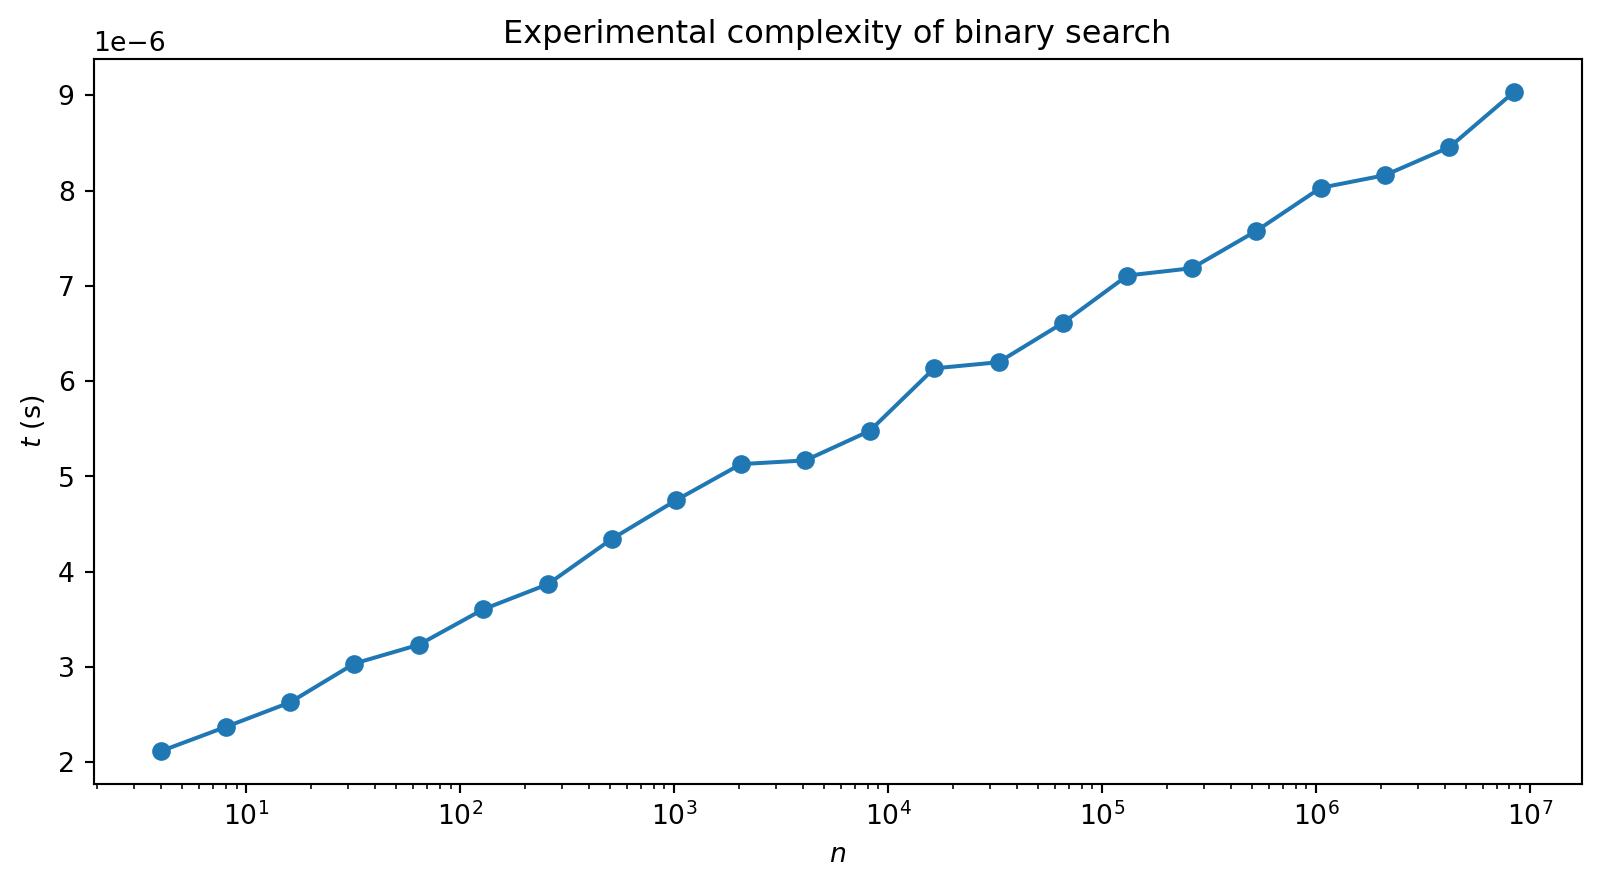
\includegraphics{./ode_files/figure-pdf/cell-5-output-1.pdf}

}

\end{figure}

The thickness of the blue line is due to the variation of the energy
over the \(t=1000\) trajectory (measured in units where the frequency of
linear oscillation is \(2\pi\)). Notice that we did not have to specify
a time step: this is determined \emph{adaptively} by the solver to keep
the estimate of the local error below \texttt{atol\ +\ rtol\ *\ abs(y)},
where \texttt{atol} and \texttt{rtol} are optional arguments that
correspond to the absolute and relative tolerances, with default values
of \(10^{-6}\) and \(10^{-3}\) respectively. The global error is of
course much larger. In general, monitoring conserved quantities is a
good experimental method for assessing the accuracy of integration.

The alternative to \texttt{dense\_output=True} is to track ``events'',
which are user-defined points of interest on the trajectory. We supply
\texttt{solve\_ivp} with functions \texttt{event(t,\ x)} whose zeros
define the events. We can use events to take a ``cross section'' of
higher dimensional motion. As an example let's consider the
\href{https://en.wikipedia.org/wiki/H\%C3\%A9non\%E2\%80\%93Heiles_system}{Hénon--Heiles
system}, a model chaotic system with origins in stellar dynamics

\[
\begin{align}
\dot x &= p_x \\
\dot p_x &= -x -2\lambda xy \\
\dot y &= p_y \\
\dot p_y &=  - y -\lambda(x^2-y^2).
\end{align}
\]

These coupled first order systems for the \(N\) coordinates and \(N\)
momenta of a mechanical system with \(N\) degrees of freedom are an
example of
\href{https://en.wikipedia.org/wiki/Hamiltonian_mechanics}{Hamilton's
equations}. The phase space is now four dimensional and impossible to
visualize.

The conserved energy is

\[
E = \frac{1}{2}\left(p_x^2+p_y^2 + x^2 + y^2\right) + \lambda\left(x^2y-\frac{1}{3}y^3\right)
\]

If we take a
\href{https://en.wikipedia.org/wiki/Poincar\%C3\%A9_map}{Poincaré
section} with \(x=0\) a system with energy \(E\) must lie within the
curve defined by

\[
E = \frac{1}{2}\left(p_y^2 + y^2\right) -\frac{\lambda}{3}y^3.
\]

Starting from \(x=0\) we can generate a section of given \(E\) by
solving for \(p_x\)

\[
p_x = \sqrt{2E-y^2-p_y^2 + \frac{2\lambda}{3}y^3}
\]

\begin{Shaded}
\begin{Highlighting}[]
\KeywordTok{def}\NormalTok{ henon\_heiles(t, z, 𝜆): }
\NormalTok{    x, px, y, py }\OperatorTok{=}\NormalTok{ z}
    \ControlFlowTok{return}\NormalTok{ [px, }\OperatorTok{{-}}\NormalTok{x }\OperatorTok{{-}} \DecValTok{2} \OperatorTok{*}\NormalTok{ 𝜆 }\OperatorTok{*}\NormalTok{ x }\OperatorTok{*}\NormalTok{ y, py, }\OperatorTok{{-}}\NormalTok{y }\OperatorTok{{-}}\NormalTok{ 𝜆 }\OperatorTok{*}\NormalTok{ (x}\OperatorTok{**}\DecValTok{2} \OperatorTok{{-}}\NormalTok{ y}\OperatorTok{**}\DecValTok{2}\NormalTok{)]}

\KeywordTok{def}\NormalTok{ px(E, y, py, 𝜆):}
    \ControlFlowTok{return}\NormalTok{ np.sqrt(}\DecValTok{2} \OperatorTok{*}\NormalTok{ E }\OperatorTok{{-}}\NormalTok{ y}\OperatorTok{**}\DecValTok{2} \OperatorTok{{-}}\NormalTok{ py}\OperatorTok{**}\DecValTok{2} \OperatorTok{+} \DecValTok{2} \OperatorTok{*}\NormalTok{ 𝜆 }\OperatorTok{*}\NormalTok{ y}\OperatorTok{**}\DecValTok{3} \OperatorTok{/} \DecValTok{3}\NormalTok{)}

\KeywordTok{def}\NormalTok{ section(t, y, 𝜆): }\ControlFlowTok{return}\NormalTok{ y[}\DecValTok{0}\NormalTok{] }\CommentTok{\# The section with x=0}

\NormalTok{t\_max }\OperatorTok{=} \DecValTok{10000}
\NormalTok{𝜆 }\OperatorTok{=} \DecValTok{1}
\NormalTok{hh\_motion }\OperatorTok{=}\NormalTok{ []}
\ControlFlowTok{for}\NormalTok{ E }\KeywordTok{in}\NormalTok{ [}\DecValTok{1}\OperatorTok{/}\DecValTok{12}\NormalTok{, }\DecValTok{1}\OperatorTok{/}\DecValTok{8}\NormalTok{, }\DecValTok{1}\OperatorTok{/}\DecValTok{6}\NormalTok{]:}
\NormalTok{    hh\_motion.append(solve\_ivp(henon\_heiles, [}\DecValTok{0}\NormalTok{, t\_max], [}\DecValTok{0}\NormalTok{, px(E, }\FloatTok{0.1}\NormalTok{, }\FloatTok{0.1}\NormalTok{, 𝜆), }\FloatTok{0.1}\NormalTok{, }\FloatTok{0.1}\NormalTok{], events}\OperatorTok{=}\NormalTok{section, args}\OperatorTok{=}\NormalTok{[𝜆], atol}\OperatorTok{=}\FloatTok{1e{-}7}\NormalTok{, rtol}\OperatorTok{=}\FloatTok{1e{-}7}\NormalTok{))}
\end{Highlighting}
\end{Shaded}

We can then plot a section of the phase space with increasing energy,
showing the transition from regular to chaotic dynamics.

\begin{Shaded}
\begin{Highlighting}[]
\NormalTok{fig, ax }\OperatorTok{=}\NormalTok{ plt.subplots(}\DecValTok{1}\NormalTok{, }\DecValTok{3}\NormalTok{)}
\NormalTok{energies }\OperatorTok{=}\NormalTok{ [}\StringTok{"1/12"}\NormalTok{, }\StringTok{"1/8"}\NormalTok{, }\StringTok{"1/6"}\NormalTok{]}
\ControlFlowTok{for}\NormalTok{ idx, data }\KeywordTok{in} \BuiltInTok{enumerate}\NormalTok{(hh\_motion): }
\NormalTok{        ax[idx].scatter(}\OperatorTok{*}\NormalTok{data.y\_events[}\DecValTok{0}\NormalTok{][:, }\DecValTok{2}\NormalTok{:].T, s}\OperatorTok{=}\FloatTok{0.1}\NormalTok{)}
\NormalTok{        ax[idx].title.set\_text(}\SpecialStringTok{f"E=}\SpecialCharTok{\{}\NormalTok{energies[idx]}\SpecialCharTok{\}}\SpecialStringTok{"}\NormalTok{)        }
\NormalTok{        ax[idx].set\_xlabel(}\VerbatimStringTok{r\textquotesingle{}$y$\textquotesingle{}}\NormalTok{)}

\NormalTok{ax[}\DecValTok{0}\NormalTok{].set\_ylabel(}\VerbatimStringTok{r\textquotesingle{}$p\_y$\textquotesingle{}}\NormalTok{)}
\NormalTok{plt.show()}
\end{Highlighting}
\end{Shaded}

\begin{figure}[H]

{\centering 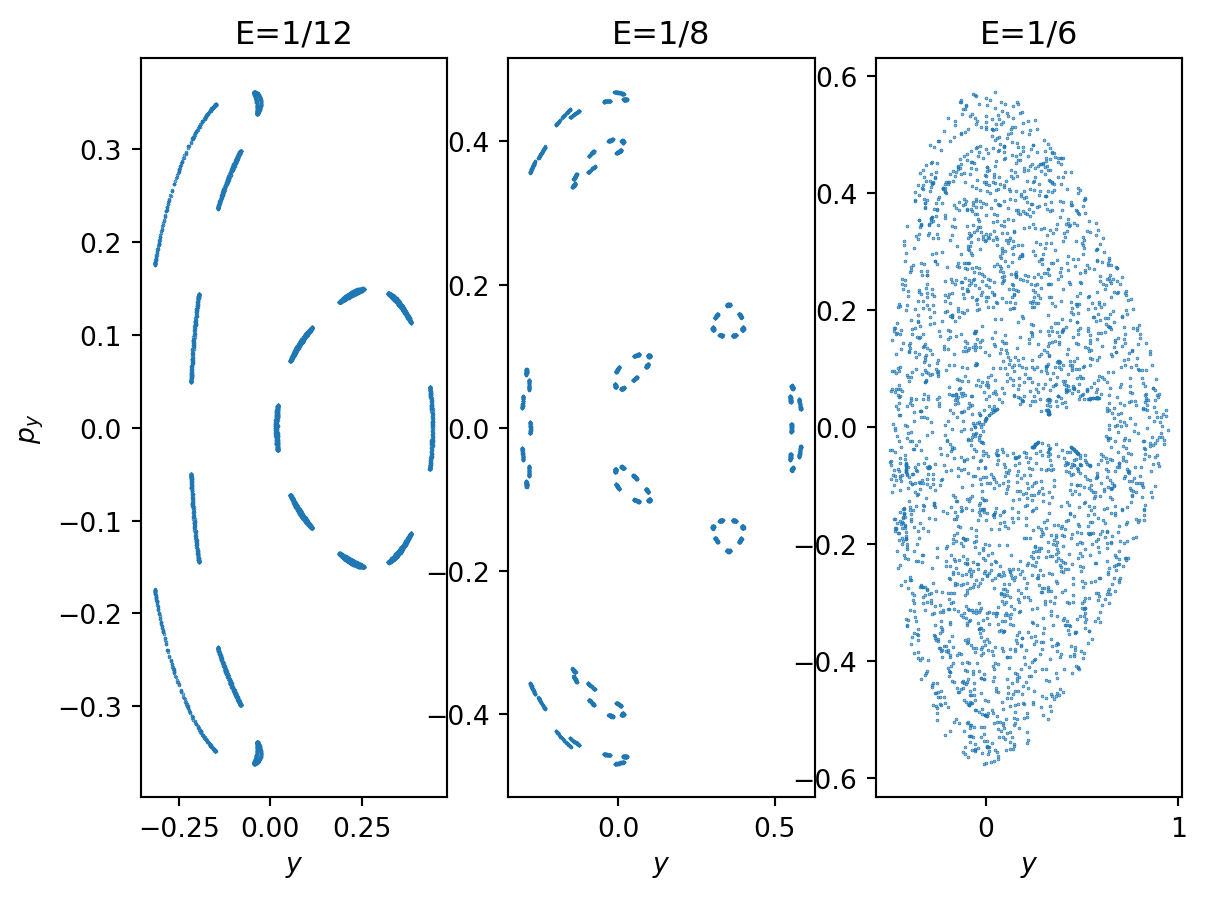
\includegraphics{./ode_files/figure-pdf/cell-7-output-1.pdf}

}

\end{figure}

TODO Leapfrog?

\href{https://duetosymmetry.com/tool/poincare-section-clicker-toy/}{Nice
demo on Poincaré sections}

Symplectic integrator see e.g.~

Look at leapfrog?

https://github.com/scipy/scipy/issues/12690

Problem is that it's hard to do in scipy

https://stackoverflow.com/questions/60338471/lyapunov-spectrum-for-known-odes-python-3

\bookmarksetup{startatroot}

\hypertarget{monte-carlo-methods}{%
\chapter{Monte Carlo methods}\label{monte-carlo-methods}}

Many physical phenomena, notably those falling within the domains of
statistical mechanics and quantum theory, depend in an essential way on
\emph{randomness}. The simulation of these phenomena therefore requires
algorithms that incorporate random (or pseudo-random) elements in the
most efficient way.

\hypertarget{sampling-from-a-distribution}{%
\section{Sampling from a
distribution}\label{sampling-from-a-distribution}}

Let's suppose that we have a source of samples of a real valued random
variable \(X\) that follows a particular probability density function
\(p_X\) \footnote{Sticking with integers} (more about where they might
come from in Section~\ref{sec-rng}). This means that the probability of
drawing a sample in the region \([x, x+dx]\) is \(p_X(x)dx\). If we now
map the samples using a function \(f\), what is the probability density
\(p_Y\) of \(y=f(x)\)? The new probability density is defined in just
the same way: the probability of \(y\) lying in the region \([y, y+dy]\)
is \(p_Y(y)dy\). Since \(x\) is being mapped deterministically to \(y\)
these two probabilities are therefore the same

\[
p_X(x)dx = p_Y(y)dy
\]

or

\[
p_Y(y)=p_X(x)\Bigg\lvert \frac{dx}{dy}\Bigg\rvert= \frac{p_X(x)}{|f'(x)|},\qquad x=f^{-1}(y)
\]

This formula shows that we can create samples from an arbitrary
probability distribution by choosing an invertible map \(f\)
appropriately. If \(p_X\) is a
\href{https://en.wikipedia.org/wiki/Continuous_uniform_distribution}{standard
uniform distribution} on \([0,1]\) then \(f(x)\) is the inverse of the
cummulative probability distribution of \(Y\) i.e.

\[
f^{-1}(y) = \int^y_{-\infty} p_Y(y')dy'
\]

The same approach works in higher dimensions:
\(\big\lvert \frac{dx}{dy}\big\rvert\) is replaced by the inverse of the
Jacobian determinant.

The
\href{https://en.wikipedia.org/wiki/Box\%E2\%80\%93Muller_transform}{Box--Muller
transform} is one example of this idea. Take two independent samples
from a standard uniform distribution \(u_{1,2}\) and form

\[
\begin{align}
x &= \sqrt{-2\log u_1}\cos(2\pi u_2)\\
y &= \sqrt{-2\log u_1}\sin(2\pi u_2).
\end{align}
\]

\(x\) and \(y\) are independent samples from a
\href{https://en.wikipedia.org/wiki/Standard_normal_distribution}{standard
normal distribution}.

Various functions are available in the
\href{https://numpy.org/doc/stable/reference/random/index.html\#module-numpy.random}{\texttt{numpy.random}}
module to generate random arrays drawn from a variety of distributions.
Box--Muller has now been retired in favour of the
\href{https://en.wikipedia.org/wiki/Ziggurat_algorithm}{Ziggurat
algorithm}.

\begin{Shaded}
\begin{Highlighting}[]
\ImportTok{import}\NormalTok{ numpy.random }\ImportTok{as}\NormalTok{ random}
\ImportTok{import}\NormalTok{ numpy }\ImportTok{as}\NormalTok{ np}
\ImportTok{import}\NormalTok{ matplotlib.pyplot }\ImportTok{as}\NormalTok{ plt}

\NormalTok{mu, sigma }\OperatorTok{=} \DecValTok{0}\NormalTok{, }\FloatTok{0.1} \CommentTok{\# mean and standard deviation}
\NormalTok{s }\OperatorTok{=}\NormalTok{ random.normal(mu, sigma, size}\OperatorTok{=}\DecValTok{10000}\NormalTok{)}
\NormalTok{count, bins, ignored }\OperatorTok{=}\NormalTok{ plt.hist(s, }\DecValTok{30}\NormalTok{, density}\OperatorTok{=}\VariableTok{True}\NormalTok{)}
\NormalTok{plt.plot(bins, }\DecValTok{1}\OperatorTok{/}\NormalTok{(sigma }\OperatorTok{*}\NormalTok{ np.sqrt(}\DecValTok{2} \OperatorTok{*}\NormalTok{ np.pi)) }\OperatorTok{*}
\NormalTok{               np.exp( }\OperatorTok{{-}}\NormalTok{ (bins }\OperatorTok{{-}}\NormalTok{ mu)}\OperatorTok{**}\DecValTok{2} \OperatorTok{/}\NormalTok{ (}\DecValTok{2} \OperatorTok{*}\NormalTok{ sigma}\OperatorTok{**}\DecValTok{2}\NormalTok{) ),}
\NormalTok{         linewidth}\OperatorTok{=}\DecValTok{2}\NormalTok{, color}\OperatorTok{=}\StringTok{\textquotesingle{}r\textquotesingle{}}\NormalTok{)}
\NormalTok{plt.xlabel(}\StringTok{"Value"}\NormalTok{)}
\NormalTok{plt.ylabel(}\StringTok{"Frequency"}\NormalTok{)}
\NormalTok{plt.show()}
\end{Highlighting}
\end{Shaded}

\begin{figure}[H]

{\centering \includegraphics{./monte-carlo_files/figure-pdf/cell-2-output-1.pdf}

}

\end{figure}

For complex multivariate (i.e.~high dimensional) distributions there is
no general recipe to construct an appropriate \(f\). One very recent
application of these ideas is in machine learning models called
\href{https://arxiv.org/abs/1908.09257}{normalizing flows} that use a
mapping \(f\) parameterized by a neural network. The workhorse for
sampling from complicated distributions is Markov chain Monte Carlo, as
we discuss in Section~\ref{sec-mcmc}.

\hypertarget{the-monte-carlo-method}{%
\section{The Monte Carlo method}\label{the-monte-carlo-method}}

\emph{Monte Carlo} is the general prefix applied to variety of numerical
methods that use randomness in some way. Two of the main classes of
problem encountered in physics that come under this heading are:

\begin{enumerate}
\def\labelenumi{\arabic{enumi}.}
\item
  Interpret a numerical evaluation as an expectation value of some
  random variable and use sampling to estimate it.
  \href{https://en.wikipedia.org/wiki/Monte_Carlo_integration}{Monte
  Carlo integration} is an example of this idea.
\item
  Sampling from a complex probability distribution (which may include
  taking expectation values). Example:
  \href{https://en.wikipedia.org/wiki/Markov_chain_Monte_Carlo}{Markov
  chain Monte Carlo}.
\end{enumerate}

\hypertarget{monte-carlo-integration}{%
\subsection{Monte Carlo integration}\label{monte-carlo-integration}}

The technique is exemplified by the following fairly dumb way of
estimating \(\pi\)

\begin{Shaded}
\begin{Highlighting}[]
\NormalTok{max\_samples }\OperatorTok{=} \DecValTok{10000}
\NormalTok{inside }\OperatorTok{=} \DecValTok{0}
\NormalTok{areas }\OperatorTok{=}\NormalTok{ []}
\ControlFlowTok{for}\NormalTok{ sample }\KeywordTok{in} \BuiltInTok{range}\NormalTok{(}\DecValTok{1}\NormalTok{, max\_samples }\OperatorTok{+} \DecValTok{1}\NormalTok{):}
\NormalTok{    x }\OperatorTok{=}\NormalTok{ random.uniform(}\OperatorTok{{-}}\DecValTok{1}\NormalTok{, }\DecValTok{1}\NormalTok{)}
\NormalTok{    y }\OperatorTok{=}\NormalTok{ random.uniform(}\OperatorTok{{-}}\DecValTok{1}\NormalTok{, }\DecValTok{1}\NormalTok{)}
    
    \ControlFlowTok{if}\NormalTok{ x }\OperatorTok{**} \DecValTok{2} \OperatorTok{+}\NormalTok{ y }\OperatorTok{**} \DecValTok{2} \OperatorTok{\textless{}=} \DecValTok{1}\NormalTok{:}
\NormalTok{        inside }\OperatorTok{+=} \DecValTok{1}
\NormalTok{    areas.append(}\DecValTok{4} \OperatorTok{*}\NormalTok{ inside }\OperatorTok{/}\NormalTok{ sample)}

\NormalTok{plt.plot(np.arange(}\DecValTok{1}\NormalTok{, max\_samples }\OperatorTok{+} \DecValTok{1}\NormalTok{), areas)}
\NormalTok{plt.plot(np.arange(}\DecValTok{1}\NormalTok{, max\_samples }\OperatorTok{+} \DecValTok{1}\NormalTok{), np.pi }\OperatorTok{*}\NormalTok{ np.ones(max\_samples), linestyle}\OperatorTok{=}\StringTok{\textquotesingle{}dashed\textquotesingle{}}\NormalTok{)}
\NormalTok{plt.show()}
\end{Highlighting}
\end{Shaded}

\begin{figure}[H]

{\centering 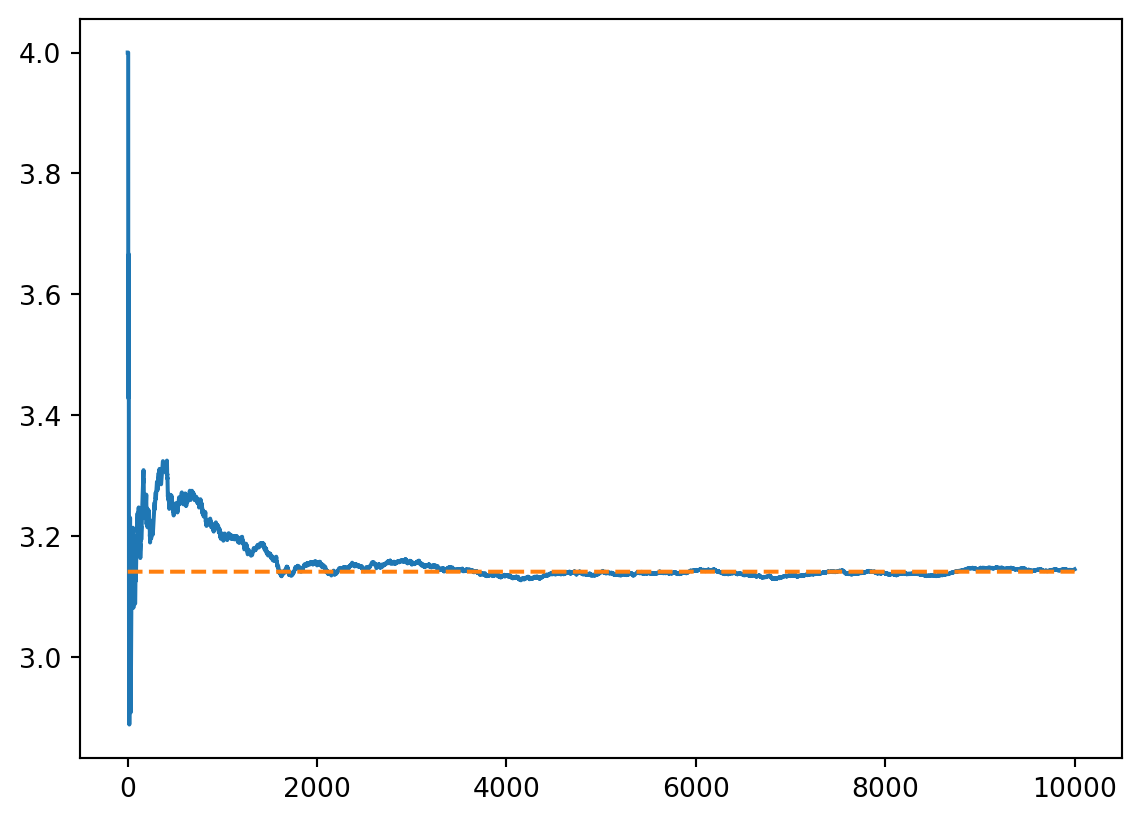
\includegraphics{./monte-carlo_files/figure-pdf/cell-3-output-1.pdf}

}

\end{figure}

In terms of integration, you can think of this as a way to compute the
integral of a function which is one inside the unit disc, and zero
outside it.

Although it's a silly method, this does illustrate one important feature
of Monte Carlo methods in general: that the relative error with \(N\)
samples is typically \(\propto N^{-1/2}\) (thus at the 1\% level for
\(10^4\) samples) because the variance of a sum of \(N\)
\href{https://en.wikipedia.org/wiki/Independent_and_identically_distributed_random_variables}{iid}
variables is \(\propto N^{1/2}\).

TODO General setting. Importance sampling

Monte Carlo integration comes into its own for high dimensional
problems. For low dimensional integrals the quadrature methods in
\href{https://docs.scipy.org/doc/scipy/tutorial/integrate.html}{\texttt{scipy.integrate}}
are preferable.

\hypertarget{sec-mcmc}{%
\subsection{Markov chain Monte Carlo}\label{sec-mcmc}}

Suppose you want to generate configurations at random (i.e.~with a
uniform distribution) from a ``gas'' of hard disks \footnote{I've
  borrowed this example from
  \href{https://github.com/CambridgeEngineering/PartIA-Computing-Michaelmas/blob/main/11\%20Complexity.ipynb}{Garth
  Wells' course}}.

\begin{figure}

{\centering 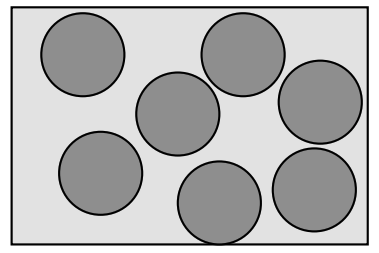
\includegraphics{./assets/hard-spheres.png}

}

\caption{Coins in a shoe box (gas of hard disks). From Krauth (1998)}

\end{figure}

It's harder than it looks! The first guess you might have is to start
adding coins at random, and if you get an overlap, try again until you
don't. Obviously this will become inefficient as the box fills up, and
most attempts fail. \emph{Worse, it doesn't in fact yield a uniform
distribution!}

TODO Why not? See Widom (1966) for an explanation

Here's an approach that works:

\leavevmode\vadjust pre{\hypertarget{exm-metropolis}{}}%
\begin{example}[Metropolis algorithm for hard
disks]\label{exm-metropolis}

~

\begin{enumerate}
\def\labelenumi{\arabic{enumi}.}
\tightlist
\item
  Fix the number of disks and an initial configuration (some regular
  lattice configuration, say).
\item
  Pick a disk at random and attempt (or \emph{propose}) to move it by a
  small random amount (i.e.~random direction; random small magnitude).
\item
  If this results in the moved disk intersecting another, \emph{reject}
  the move, leaving the disk where it is. Otherwise, \emph{accept} the
  move.
\item
  Repeat 2. and 3. many times.
\end{enumerate}

\end{example}

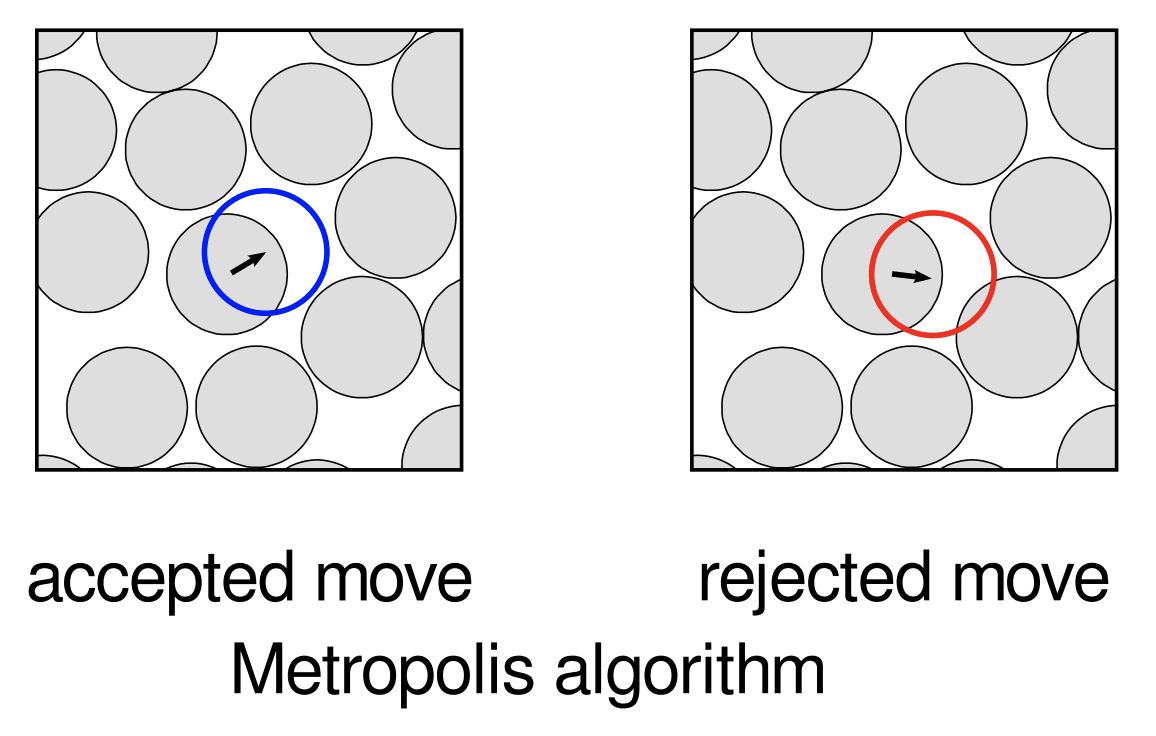
\includegraphics{./assets/metropolis.png}.

TODO js demo

This is the simplest example of the
\href{https://en.wikipedia.org/wiki/Metropolis\%E2\%80\%93Hastings_algorithm}{Metropolis--Hastings
algorithm}, the first Markov chain Monte Carlo (MCMC) algorithm.

More generally, the goal of MCMC is to come up with a sequential random
process (a \textbf{Markov chain}) that generates (usually after many
steps) a sample from a particular distribution.

You've all heard of a
\href{https://en.wikipedia.org/wiki/Random_walk}{random walk}, perhaps
as a model for diffusion. At each step you make a move in a random
direction, independently of your earlier moves. After many steps these
random moves gives rise to a distribution of possible locations. A
random walk is the simplest example of a Markov chain.

More generally, a
\href{https://en.wikipedia.org/wiki/Markov_chain}{Markov chain} is a
sequence of random variables \(X_n\) with each having a distribution
that is is conditional on the value of the previous one, and so is
defined in terms of \textbf{transition probabilities}
\(p(X_{n}=x_n|X_{n-1}=x_{n-1})\) (hence they form a ``chain''). I'm
going to immediately drop this cumbersome notation in favour of
\(p(x_n|x_{n-1})\), a function of \(x_n\) and \(x_{n-1}\), but in
general the function giving the transition probabilities can be
different at each step (the random variables could all be different).

The probability of a particular sequence \(X_1=x_1\ldots X_n=x_n\) is
therefore

\[
p(x_n|x_{n-1})p(x_{n-1}|x_{n-2})\cdots p(x_2|x_{1})p^{(1)}(x_1)
\]

\(X_1\) has no ``parent'' so is not conditional on any other value.

Suppose we don't care about the earlier values and just want to know the
\textbf{marginal distribution} \(p^{(n)}(x_n)\) of the final variable.
For a random walk this is easy, as \(x_n\) typically represents a
displacement that is a sum of iid increments. In general this is not the
case, however, as the marginal distribution is

\[
p^{(n)}(x_n)=\sum_{x_{n-1},\ldots x_1}p(x_n|x_{n-1})p(x_{n-1}|x_{n-2})\cdots p(x_2|x_{1})p^{(1)}(x_1)
\]

(I'm writing all these expressions for discrete random variables, but
the continuous version involving probability density functions is
straightforward)

The sums are over all possible values that the random variables might
take in the \textbf{state space} of the problem. These could be finite
or infinite in number.

Things are not as bad as they appear, however, as the marginal
distribution can be interpreted as the result of acting \(n-1\) times on
the vector of values of \(p^{(1)}_j\equiv p^{(1)}(j)\) with the
\textbf{transition matrix} with elements \(\mathsf{P}_{jk}=p(j|k)\)

\[
\mathbf{p}^{(n)} = \mathsf{P}^{n-1}\mathbf{p}^{(1)}.
\]

In a single step the marginal probabilities are updated as

\[
\mathbf{p}^{(n)} = \mathsf{P}^{n}\mathbf{p}^{(n-1)}.
\]

\(\mathsf{P}\) has some structure. The matrix elements are positive, as
they represent probabilities, and each row sums to one

\[
\sum_j \mathsf{P}_{jk} = 1.
\]

Such matrices are called
\href{https://en.wikipedia.org/wiki/Stochastic_matrix}{stochastic}.

Although \(p^{(n)}\) --- the probability distribution at the \(n\)th
step --- changes from step to step, you might expect that after many
steps it tends to converge to a \textbf{stationary distribution}
\(p^{(n)}\to\boldsymbol{\pi}\). If it exists, this distribution must
satisfy

\begin{equation}\protect\hypertarget{eq-stat}{}{
\boldsymbol{\pi} = \mathsf{P}\boldsymbol{\pi}.
}\label{eq-stat}\end{equation}

In other words, it is an eigenvector of \(\mathsf{P}\) with eigenvalue
one. This property is guaranteed by the
\href{https://en.wikipedia.org/wiki/Perron\%E2\%80\%93Frobenius_theorem}{Perron--Frobenius
theorem} \footnote{\href{https://en.wikipedia.org/wiki/Grover\%27s_algorithm}{Grover's
  algorithm} for search has \(O(\sqrt{n})\) complexity, but there's a
  catch: you need a \emph{quantum computer}, and even then a
  \(\sqrt{n}\) speedup is not going to get you a billion dollars in this
  economy.}.

Thus \(\mathsf{P}\) determines \(\boldsymbol{\pi}\). MCMC turns this
idea on its head and asks: if there is some \(\boldsymbol{\pi}\) that I
would like to generate samples from, can I find a \(\mathsf{P}\) that
has it as a stationary distribution?

There is a trivial answer to this question. Sure, take
\(\mathsf{P}_{jk}=\boldsymbol{\pi}_j\). That is, jump straight to the
stationary distribution no matter what the starting state. But we are
interested in highly complicated distributions over large state spaces
(think the Boltzmann distribution for a statistical mechanical system
comprised of billions of particles). Thus what we really want is to be
able to approach such a complicated distribution by making many
transitions with \emph{simple} distributions.

One more idea is useful before returning to concrete algorithms. The
quantity

\[
\mathsf{P}_{jk}\pi_k = p(j|k)\pi_k = p(j,k)
\]

is the joint distribution of seeing state \(k\) followed by state \(j\)
in the stationary distribution. A \emph{reversible} Markov chain is one
where \(p(j,k)=p(k,j)\). Roughly, you can't tell the direction of time
because any transition is equally likely to happen forward in time as
backward. Random physical processes that respect time reversal symmetry
are often modeled as reversible Markov processes.

Combining reversibility with the definition of the stationary state
yields the condition of
\href{https://en.wikipedia.org/wiki/Detailed_balance}{detailed balance}

\begin{equation}\protect\hypertarget{eq-detailed}{}{
 \mathsf{P}_{jk}\pi_k = \pi_j\mathsf{P}_{kj}.
}\label{eq-detailed}\end{equation}

This condition is stronger than the condition Equation~\ref{eq-stat} for
a stationary state. This makes it easier to check: you don't have to do
a sum over a state space index. The Metropolis algorithm
Example~\ref{exm-metropolis} for the hard disk problem satisfies
detailed balance for a stationary distribution that is constant when
disks don't intersect and zero when they do.

When the stationary distribution \(\boldsymbol{\pi}\) has more
structure, designing an appropriate transition matrix is harder. The
idea is to generalize the hard disk approach by separating the
transition into a \emph{proposal} distribution \(p_\text{prop}(j|k)\)
and an \emph{acceptance} distribution
\(p_\text{acc}(a=0,1|j\leftarrow k)\) that gives the probability of a
move from \(k\) to \(j\) being accepted (\(a=1\)) or rejected (\(a=0\)).
The probability of moving from \(k\) to \(j\) is then

\[
p(j|k) = p_\text{acc}(a=1|j\leftarrow k) p_\text{prop}(j|k).
\]

Substituting this into the detailed balance condition
Equation~\ref{eq-detailed} gives \[
\frac{p_\text{acc}(a=1|j\leftarrow k)}{p_\text{acc}(a=1|k\leftarrow j)} = \frac{\pi_j}{\pi_k}\frac{p_\text{prop}(k|j)}{p_\text{prop}(j|k)}.
\]

Any \(p_\text{acc}\) that satisfies this relation for all \(j\) and
\(k\) will do the job. The Metropolis choice is

\begin{equation}\protect\hypertarget{eq-metropolis}{}{
p_\text{acc}(a=1|j \leftarrow k) = \min\left(1,  \frac{\pi_j}{\pi_k}\frac{p_\text{prop}(k|j)}{p_\text{prop}(j|k)}\right).
}\label{eq-metropolis}\end{equation}

This gives an extremely general algorithm, one of the top ten in applied
mathematics, according to
\href{https://nhigham.com/2016/03/29/the-top-10-algorithms-in-applied-mathematics/}{one
list}:

\leavevmode\vadjust pre{\hypertarget{exm-metropolis-gen}{}}%
\begin{example}[Metropolis algorithm]\label{exm-metropolis-gen}

~

\begin{enumerate}
\def\labelenumi{\arabic{enumi}.}
\tightlist
\item
  Starting from state \(k\) sample a next state \(j\) from the proposal
  distribution \(p_\text{prop}(j|k)\).
\item
  Accept the proposal with probability
  \(p_\text{acc}(a=1|j \leftarrow k)\) and move to state \(j\).
  Otherwise reject the proposal and stay in state \(k\).
\item
  Repeat 1. and 2. many times.
\end{enumerate}

\end{example}

MCMC has the benefit of being
\href{https://en.wikipedia.org/wiki/Embarrassingly_parallel}{embarrassingly
parallel}. If you want to average something over \(\boldsymbol{\pi}\),
just run the algorithm many times independently and average the results.
This is perfect for parallel computing.

The Metropolis algorithm has an Achilles' heel, however. To perform a
move one has to sample from \(p_\text{prop}(j|k)\) and from
\(p_\text{acc}(a|j \leftarrow k)\). The proposal therefore has to be
tractable, like the small shift in position for the hard disk case. This
may however, mean that that many of the \(j\)s suggested correspond to
very small \(\pi_j\), and therefore a very low acceptance probability
(c.f. Equation~\ref{eq-metropolis}). For example, in the hard disk case
at high density many proposed moves will give rise to overlap of disks
and be rejected. This means that many steps are required to have one
successful update of the simulation. This kind of slowdown is a common
feature of MCMC methods applied to complex distributions.

We'll see some more examples of MCMC algorithms for statistical
mechanical problems in Section~\ref{sec-statmech}, and ways in which
this problem can be avoided.

\hypertarget{relaxation-to-equilibrium}{%
\subsection{Relaxation to equilibrium}\label{relaxation-to-equilibrium}}

Eigenvalues

Master equation

Transition matrix

\hypertarget{sec-statmech}{%
\section{Statistical mechanics}\label{sec-statmech}}

Statistical mechanics is a natural source of such complex distributions
in physics. Remember the fundamental principle that the probability of
finding a statistical mechanical system in a microstate \(\mathbf{x}\)
\footnote{For a classical gas of point particles this would correspond
  to specifying all the positions and velocities, for example.} with
energy \(\mathcal{E}(\mathbf{x})\) is

\begin{equation}\protect\hypertarget{eq-boltzmann}{}{
p(\mathbf{x})=\frac{\exp\left[-\beta \mathcal{E}(\mathbf{x})\right]}{Z},
}\label{eq-boltzmann}\end{equation}

where \(Z\) is a normalizing constant called the partition function and
\(\beta=1/k_\text{B}T\), where \(T\) is the temperature and
\(k_\text{B}\) is Boltzmann's constant.

The \emph{central problem} of statistical mechanics is computing
ensemble averages of physical quantities, and the \emph{principle
difficulty} is the intractability of those averages for large systems.
For example, if we are dealing with a classical gas, the configuration
space point \(\mathbf{x}\) corresponds to the positions of each of the
gas molecules \(\mathbf{x}=(\mathbf{x}_1,\ldots \mathbf{x}_N)\) and an
average is a \(3N\)-dimensional integral. The only situation in which
this integral is tractable is when the gas is noninteracting (ideal), in
which case the energy function takes the form

\[
\mathcal{E}(\mathbf{x}) = \sum_{n=1}^N \mathcal{E}_1(\mathbf{x}_n)
\]

where \(\mathcal{E}_1(\mathbf{x})\) is the single particle energy. In
this case the integral factorizes. As soon as we introduce interactions
between particles of the form

\[
\mathcal{E}(\mathbf{x}) = \sum_{n<m}^N \mathcal{E}_2(\mathbf{x}_n,\mathbf{x}_m)
\]

things get a lot harder. The same issue arises in models involving
discrete random variables. The canonical example is the
\href{https://en.wikipedia.org/wiki/Ising_model}{Ising model}, in which
a configuration corresponds to fixing the values of \(N\) ``spins''
\(\sigma_n=\pm 1\) with an energy function of the form

\[
\mathcal{E}(\sigma)=\sum_n h_n\sigma_n + \sum_{m<n} J_{mn}\sigma_m\sigma_n.
\]

The two terms correspond to a (magnetic) field that acts on each spin
and a coupling between spins. As in the gas, it's the latter that causes
problems / interest.

The Ising model comes in a great many flavours according to how the
fields and couplings are chosen. They may reflect a lattice structure:
\(J_{mn}\neq 0\) for nearest neighbours, say, or longer range. They may
be fixed or random, defining an ensemble of models.

The most pessimistic assessment is that to calculate an average we are
going to have sum over \(2^N\) configurations. Computing the partition
function \(Z\) that normalizes the average (or which gives the free
energy via \(F=-k_\text{B}T\log Z\)) is another such sum.

Monte Carlo simulation is a much more attractive alternative. MCMC can
be used to generate samples from \(p(\sigma)\) which are then used to
estimate the averages of interest (e.g.~average energy
\(\langle\mathcal{E}(\sigma)\rangle\), average magnetization
\(\langle\sum_n \sigma_n\rangle\), etc.).

\hypertarget{mcmc-updates-for-the-ising-model}{%
\subsection{MCMC updates for the Ising
model}\label{mcmc-updates-for-the-ising-model}}

How does MCMC work in practice for the Ising model? To apply the
Metropolis alogorithm Example~\ref{exm-metropolis-gen} we can use a
simple proposal: pick each spin in turn in some order and try to flip
it.

The form of \(p(\sigma)\) means that, although we cannot compute the
probabilities explicitly, we can calculate \emph{ratios}, which is all
we need for Metropolis. For two configurations that differ only by
\(\sigma_n=\pm 1\) we have

\[
\begin{align}
\frac{p(\sigma_n=1|\sigma_{m\neq n})}{p(\sigma_n=-1|\sigma_{m\neq n})} &= \exp\left[-2\beta \left(h_n+\sum_{m\neq n} J_{mn}\sigma_m\right)\right]\\
&\equiv \exp\left[-\beta\Delta \mathcal{E}\right],
\end{align}
\]

where \(\Delta \mathcal{E}\) is the energy difference between two
configurations.

One alternative to Metropolis is the \textbf{Heat bath algorithm} (or
\href{https://en.wikipedia.org/wiki/Glauber_dynamics}{Glauber dynamics}
or \href{https://en.wikipedia.org/wiki/Gibbs_sampling}{Gibbs sampling})
\footnote{Multiple names are sign that a technique was re-discovered by
  different communities who don't talk to each other.}. The idea behind
the name is that, since we can calculate the influence of the spin's
environment (the ``bath''), we can just choose the spin's orientation
with the corresponding probabilities. Since there are only two
probabilities the ratio is all we need and we get

\begin{equation}\protect\hypertarget{eq-heat-bath}{}{
p(\sigma_n=\pm 1|\sigma_{m\neq n}) = \frac{1}{1+ e^{\pm\beta \Delta \mathcal{E}}}.
}\label{eq-heat-bath}\end{equation}

The algorithm is then:

\leavevmode\vadjust pre{\hypertarget{exm-heat-bath}{}}%
\begin{example}[Heat bath algorithm]\label{exm-heat-bath}

~

\begin{enumerate}
\def\labelenumi{\arabic{enumi}.}
\tightlist
\item
  Pick a spin \(n\). \footnote{This can be done deterministically
    (e.g.~sequentially or in alternating blocks when the model is
    defined on a
    \href{https://en.wikipedia.org/wiki/Bipartite_graph}{bipartite
    graph}) --- which is what is normally called Gibbs sampling --- or
    at random, which corresponds to Glauber dynamics.}
\item
  Compute \(\Delta E\), the energy difference between
  \(\sigma_n=\pm 1\).
\item
  Set \(\sigma_n=\pm 1\) with probabilities given by
  Equation~\ref{eq-heat-bath}.
\item
  Repeat 1-3 many times
\end{enumerate}

\end{example}

What happens if we try and come up with more complicated proposals,
flipping many spins at once? For Metropolis, the problem is that without
a cleverly designed proposal we will be suggesting moves that are likely
to be rejected. For the heat bath algorithm, the more spins we flip, the
more complicated the evaluation of the corresponding probabilities
(\(2^n\) outcomes if we flip \(n\) spins).

The good news is that we \emph{can} do better --- much better --- than
the above algorithms. The
\href{https://en.wikipedia.org/wiki/Wolff_algorithm}{Wolff algorithm} is
one example. This proposes a cluster of spins of the same orientation to
be flipped by adding adjacent spins to an initially random chosen spin
with probability \(p_\text{add}\). It turns out that for the nearest
neighbour Ising model with Ferromagnetic coupling \(J<0\) the ``magic''
value \(p_\text{add}=1-e^{2\beta J}\) is \emph{rejection free}: the
probability to flip the whole cluster is always one. This makes for an
extremely fast algorithm that is not subject to the usual \emph{critical
slowing down} at phase transitions.

\begin{Shaded}
\begin{Highlighting}[]
\KeywordTok{class}\NormalTok{ IsingModel:}
    \KeywordTok{def} \FunctionTok{\_\_init\_\_}\NormalTok{(}\VariableTok{self}\NormalTok{, L):}
        \VariableTok{self}\NormalTok{.L }\OperatorTok{=}\NormalTok{ L}
        \VariableTok{self}\NormalTok{.spins }\OperatorTok{=}\NormalTok{ np.random.choice(a}\OperatorTok{=}\NormalTok{[}\DecValTok{1}\NormalTok{, }\OperatorTok{{-}}\DecValTok{1}\NormalTok{], size}\OperatorTok{=}\NormalTok{(L, L))}
\NormalTok{        stagger }\OperatorTok{=}\NormalTok{ np.empty(}\VariableTok{self}\NormalTok{.L, dtype }\OperatorTok{=} \BuiltInTok{bool}\NormalTok{)}
\NormalTok{        stagger[::}\DecValTok{2}\NormalTok{] }\OperatorTok{=} \VariableTok{True}
\NormalTok{        stagger[}\DecValTok{1}\NormalTok{::}\DecValTok{2}\NormalTok{] }\OperatorTok{=} \VariableTok{False}
        \VariableTok{self}\NormalTok{.mask }\OperatorTok{=}\NormalTok{ np.logical\_xor(stagger[:, np.newaxis], stagger[np.newaxis, :])}

    \KeywordTok{def}\NormalTok{ gibbs\_update(}\VariableTok{self}\NormalTok{, beta, sublattice):}
\NormalTok{        fields }\OperatorTok{=}\NormalTok{ np.roll(}\VariableTok{self}\NormalTok{.spins, }\DecValTok{1}\NormalTok{, }\DecValTok{0}\NormalTok{) }\OperatorTok{+}\NormalTok{ np.roll(}\VariableTok{self}\NormalTok{.spins, }\OperatorTok{{-}}\DecValTok{1}\NormalTok{, }\DecValTok{0}\NormalTok{) }\OperatorTok{+}\NormalTok{ np.roll(}\VariableTok{self}\NormalTok{.spins, }\DecValTok{1}\NormalTok{, }\DecValTok{1}\NormalTok{) }\OperatorTok{+}\NormalTok{ np.roll(}\VariableTok{self}\NormalTok{.spins, }\OperatorTok{{-}}\DecValTok{1}\NormalTok{, }\DecValTok{1}\NormalTok{)}
\NormalTok{        delta\_E }\OperatorTok{=} \DecValTok{2} \OperatorTok{*}\NormalTok{ fields}
\NormalTok{        spin\_up\_probabilities }\OperatorTok{=} \DecValTok{1} \OperatorTok{/}\NormalTok{ (}\DecValTok{1} \OperatorTok{+}\NormalTok{ np.exp(}\OperatorTok{{-}}\NormalTok{ beta }\OperatorTok{*}\NormalTok{ delta\_E))}
\NormalTok{        new\_spins }\OperatorTok{=} \DecValTok{2} \OperatorTok{*}\NormalTok{ (np.random.rand(}\VariableTok{self}\NormalTok{.L, }\VariableTok{self}\NormalTok{.L) }\OperatorTok{\textless{}}\NormalTok{ spin\_up\_probabilities) }\OperatorTok{{-}} \DecValTok{1}
        \VariableTok{self}\NormalTok{.spins }\OperatorTok{=}\NormalTok{ np.choose(np.logical\_xor(sublattice, }\VariableTok{self}\NormalTok{.mask), [}\VariableTok{self}\NormalTok{.spins, new\_spins])}

    \KeywordTok{def}\NormalTok{ glauber\_update(}\VariableTok{self}\NormalTok{, beta):}
\NormalTok{        x, y }\OperatorTok{=}\NormalTok{ np.random.randint(}\VariableTok{self}\NormalTok{.L, size}\OperatorTok{=}\DecValTok{2}\NormalTok{)}
\NormalTok{        fields }\OperatorTok{=} \DecValTok{0}
        \ControlFlowTok{for}\NormalTok{ neighbour }\KeywordTok{in}\NormalTok{ [((x }\OperatorTok{+} \DecValTok{1}\NormalTok{) }\OperatorTok{\%} \VariableTok{self}\NormalTok{.L, y), ((x }\OperatorTok{{-}} \DecValTok{1}\NormalTok{) }\OperatorTok{\%} \VariableTok{self}\NormalTok{.L, y), (x, (y }\OperatorTok{+} \DecValTok{1}\NormalTok{) }\OperatorTok{\%} \VariableTok{self}\NormalTok{.L), (x, (y }\OperatorTok{{-}} \DecValTok{1}\NormalTok{) }\OperatorTok{\%} \VariableTok{self}\NormalTok{.L)]:}
\NormalTok{            fields }\OperatorTok{+=} \VariableTok{self}\NormalTok{.spins[neighbour]}
\NormalTok{        delta\_E }\OperatorTok{=} \DecValTok{2} \OperatorTok{*}\NormalTok{ fields}
\NormalTok{        spin\_up\_probability }\OperatorTok{=} \DecValTok{1} \OperatorTok{/}\NormalTok{ (}\DecValTok{1} \OperatorTok{+}\NormalTok{ np.exp(}\OperatorTok{{-}}\NormalTok{ beta }\OperatorTok{*}\NormalTok{ delta\_E))        }
        \ControlFlowTok{if}\NormalTok{ np.random.rand() }\OperatorTok{\textless{}}\NormalTok{ spin\_up\_probability:}
            \VariableTok{self}\NormalTok{.spins[x, y] }\OperatorTok{=} \DecValTok{1}
        \ControlFlowTok{else}\NormalTok{:}
            \VariableTok{self}\NormalTok{.spins[x, y] }\OperatorTok{=} \OperatorTok{{-}}\DecValTok{1}

    \KeywordTok{def}\NormalTok{ wolff\_update(}\VariableTok{self}\NormalTok{, beta):}
\NormalTok{        initial\_x, initial\_y }\OperatorTok{=}\NormalTok{ np.random.randint(}\VariableTok{self}\NormalTok{.L, size}\OperatorTok{=}\DecValTok{2}\NormalTok{)}
\NormalTok{        initial\_spin }\OperatorTok{=} \VariableTok{self}\NormalTok{.spins[initial\_x, initial\_y]}
\NormalTok{        cluster }\OperatorTok{=}\NormalTok{ deque([(initial\_x, initial\_y)])}
\NormalTok{        add\_prob }\OperatorTok{=} \DecValTok{1} \OperatorTok{{-}}\NormalTok{ np.exp(}\OperatorTok{{-}}\DecValTok{2} \OperatorTok{*}\NormalTok{ beta)}

        \ControlFlowTok{while} \BuiltInTok{len}\NormalTok{(cluster) }\OperatorTok{!=} \DecValTok{0}\NormalTok{:}
\NormalTok{            x, y }\OperatorTok{=}\NormalTok{ cluster.popleft()}
            \ControlFlowTok{if} \VariableTok{self}\NormalTok{.spins[x, y] }\OperatorTok{==}\NormalTok{ initial\_spin:}
                \VariableTok{self}\NormalTok{.spins[x, y] }\OperatorTok{*=} \OperatorTok{{-}}\DecValTok{1}
                \ControlFlowTok{for}\NormalTok{ neighbour }\KeywordTok{in}\NormalTok{ (((x }\OperatorTok{+} \DecValTok{1}\NormalTok{) }\OperatorTok{\%} \VariableTok{self}\NormalTok{.L, y), ((x }\OperatorTok{{-}} \DecValTok{1}\NormalTok{) }\OperatorTok{\%} \VariableTok{self}\NormalTok{.L, y), (x, (y }\OperatorTok{+} \DecValTok{1}\NormalTok{) }\OperatorTok{\%} \VariableTok{self}\NormalTok{.L), (x, (y }\OperatorTok{{-}} \DecValTok{1}\NormalTok{) }\OperatorTok{\%} \VariableTok{self}\NormalTok{.L)):}
                    \ControlFlowTok{if} \VariableTok{self}\NormalTok{.spins[neighbour] }\OperatorTok{==}\NormalTok{ initial\_spin:}
                        \ControlFlowTok{if}\NormalTok{ np.random.rand() }\OperatorTok{\textless{}}\NormalTok{ add\_prob:}
\NormalTok{                            cluster.append(neighbour)}
\end{Highlighting}
\end{Shaded}

\begin{figure}

{\centering 

\hypertarget{ising-simulation}{}

}

\caption{\label{fig-ising}Glauber dynamics, Block Gibbs sampling and
Wolff updates compared. Change the temperature using the slider. The
centre of the slider corresponds to the critical temperature
\(k_\text{B}T = 2|J|/\log(1+\sqrt{2})\sim 2.269|J|\).}

\end{figure}

\hypertarget{the-universe-of-monte-carlo-methods}{%
\section{The universe of Monte Carlo
methods}\label{the-universe-of-monte-carlo-methods}}

Monte Carlo simulation is a vast field with practitioners and
specialists across the natural sciences, engineering, machine learning,
and statistics. In this section I'll mention a few important topics to
give a taste of what's out there. For much more detail take a look at
Krauth (2006) and / or MacKay (2003).

Probably the biggest single issue is: how do you kow when your MCMC
simulation has reached the stationary distribution \(\boldsymbol{\pi}\)?
The pragmatic approach is to monitor the averages of interest
(magnetization, say, in the case of the Ising model) over different
simulations or over a time interval and see when they stop changing.

We've touched on the issue of the
\href{https://en.wikipedia.org/wiki/Markov_chain_mixing_time}{mixing
time} in a Markov chain.

\begin{enumerate}
\def\labelenumi{\arabic{enumi}.}
\tightlist
\item
  Finite size effects
\item
  Approach to equilibrium
\item
  Critical slowing down / loss of ergodicity
\item
  Bias of estimators. Importance sampling
\end{enumerate}

Exact sampling

\href{https://en.wikipedia.org/wiki/Hamiltonian_Monte_Carlo}{Hamiltonian
Monte Carlo}.

Multispin encoding: 32 or 64 simulations Jacobs and Rebbi (1981)

https://en.wikipedia.org/wiki/Gibbs\_sampling

Other updates

A huge topic, see Krauth (2006) for much more

Also Chapter 29 of MacKay (2003)

Comment at the end about typicality

MCMC in Bayesian inference

Relation to Ising models. Community detection. Why not?

https://arxiv.org/pdf/cond-mat/0005264.pdf

Bayesian inference

\hypertarget{sec-rng}{%
\section{Random number generators}\label{sec-rng}}

Computers are deterministic

This is covered in some detail in the Nature of Computation

This is a subject dealt with already

RNGs in Trebst?

Further reading: refer to
\href{https://arxiv.org/pdf/cond-mat/9612186.pdf}{Krauth notes} or book

Other suggestions from Twitter

https://roomno308.github.io/blog/MCMC.html
https://maximilianrohde.com/posts/code-breaking-with-metropolis/

\bookmarksetup{startatroot}

\hypertarget{algorithms-and-computational-complexity}{%
\chapter{Algorithms and computational
complexity}\label{algorithms-and-computational-complexity}}

\hypertarget{first-example-multiplication}{%
\section{First example:
multiplication}\label{first-example-multiplication}}

How hard is it to multiply numbers? The bigger they are, the harder it
is, as you well know. You also know that computers are very good at
multiplying, so once you've switched from multiplying numbers yourself
to multiplying them on a computer, you may well be tempted to forget
about how hard it is. Nevertheless, computers find big numbers harder
than small numbers. How much harder?

If you remember how you learnt to multiply numbers at school, it
probably went something like this: \footnote{Sticking with integers}

\begin{longtable}[]{@{}
  >{\raggedright\arraybackslash}p{(\columnwidth - 8\tabcolsep) * \real{0.0556}}
  >{\raggedright\arraybackslash}p{(\columnwidth - 8\tabcolsep) * \real{0.0556}}
  >{\raggedright\arraybackslash}p{(\columnwidth - 8\tabcolsep) * \real{0.0556}}
  >{\raggedright\arraybackslash}p{(\columnwidth - 8\tabcolsep) * \real{0.0556}}
  >{\raggedright\arraybackslash}p{(\columnwidth - 8\tabcolsep) * \real{0.0556}}@{}}
\caption{Multiplying two 3 digit numbers}\tabularnewline
\toprule()
\begin{minipage}[b]{\linewidth}\raggedright
\end{minipage} & \begin{minipage}[b]{\linewidth}\raggedright
×
\end{minipage} & \begin{minipage}[b]{\linewidth}\raggedright
1

3
\end{minipage} & \begin{minipage}[b]{\linewidth}\raggedright
2

2
\end{minipage} & \begin{minipage}[b]{\linewidth}\raggedright
3

1
\end{minipage} \\
\midrule()
\endfirsthead
\toprule()
\begin{minipage}[b]{\linewidth}\raggedright
\end{minipage} & \begin{minipage}[b]{\linewidth}\raggedright
×
\end{minipage} & \begin{minipage}[b]{\linewidth}\raggedright
1

3
\end{minipage} & \begin{minipage}[b]{\linewidth}\raggedright
2

2
\end{minipage} & \begin{minipage}[b]{\linewidth}\raggedright
3

1
\end{minipage} \\
\midrule()
\endhead
\_

\_

3 & \_

2

6 & 1

4

9 & 2

6 & 3 \\
3 & 9 & 4 & 8 & 3 \\
\bottomrule()
\end{longtable}

For \(n\) digits we have to perform \(n^2\) single digit
multiplications. We then have to add together the \(n\) resulting
\(n\)-digit numbers. This is another \(n^2\) operations. Thus the
overall number of operations is proportional to \(n^2\): doubling the
number of digits will make the problem four times harder.

Exactly how long this takes to perform in your head or on a computer
will depend on many things, such as how long it takes you to multiply
two digits, or get the previous values out of memory (or read them of
the page), but you can't get away from the basic quadratic scaling law
of this algorithm.

\hypertarget{defining-complexity}{%
\section{Defining complexity}\label{defining-complexity}}

When computer scientists talk about the complexity of a problem, this
question of \emph{scaling of the number of steps involved} is what they
have in mind. The complexity of any particular task (or calculation) may
vary considerably --- evaluating \(100\times 100\) is considerably
easier than the general case, for example --- so instead we ask about
how a particular \emph{general} algorithm performs on a \emph{class} of
tasks. Such a class is what computer scientists mean when they talk
about a problem: multiplication of \(n\) digit numbers is a
\emph{problem}, and any particular pair of \(n\) digit numbers
represents an \emph{instance} of that problem. What we discussed above
is a particular algorithm for multiplication that has \emph{quadratic
complexity}, or ``\(O(n^2)\) complexity'' (say ``order \(n\) squared'').

This description only keeps track of how the difficulty scales with the
size of the problem. There are various reasons why this level of detail
is important:

\begin{enumerate}
\def\labelenumi{\arabic{enumi}.}
\item
  It allows us to gloss over what exactly we mean by a \emph{step}. Are
  we working in base ten or binary? Looking the digit multiplications up
  in a table or doing them from scratch?
\item
  Likewise we don't have to worry about how the algorithm is implemented
  exactly in software or hardware, what language we use, and so on.
\item
  Inevitably, we always want to look at harder and harder problems with
  bigger and bigger \(n\) (whatever \(n\) means for the problem at
  hand). If a simulation finishes for a system of length 10 we
  immediately want to run it again for length 20, and so on. It then
  becomes important to know whether our code is going to run for twice
  as long, four times as long, or \(2^{10}\) times as long (exponential
  scaling).
\end{enumerate}

\hypertarget{best-worst-average}{%
\subsection{Best / worst / average}\label{best-worst-average}}

Even when we focus on a problem in the above sense we still have to be
careful in defining the complexity of an algorithm. In general we can
characterize three complexities: best case, worse case, and average
case. To see the difference between these three consider \emph{search},
the very simple problem of finding an item in an (unordered) list of
length \(n\). How hard is this? You have to check every item until you
find the one you are looking for, so this suggests the complexity is
\(O(n)\). You could be lucky and get it first try, however, or within
the first ten tries. This means the \emph{best case complexity} of
search is \(O(1)\): it doesn't increase with the size of the problem.
The worst thing that could happen is that the sought item is last: the
\emph{worst case complexity} is \(O(n)\). On average, you'll find your
item in the middle of the list on attempt \(\sim n/2\), so the
\emph{average case complexity} is \(O(n/2)\). But this is the same as
\(O(n)\) (constants don't matter)

Thus for \emph{linear search} we have:

\begin{longtable}[]{@{}ll@{}}
\toprule()
& Complexity \\
\midrule()
\endhead
Best case & \(O(1)\) \\
Worst case & \(O(n)\) \\
Average case & \(O(n)\) \\
\bottomrule()
\end{longtable}

We can check the average case performance experimentally by using
randomly chosen lists: \footnote{I've borrowed this example from
  \href{https://github.com/CambridgeEngineering/PartIA-Computing-Michaelmas/blob/main/11\%20Complexity.ipynb}{Garth
  Wells' course}}

\begin{Shaded}
\begin{Highlighting}[]
\KeywordTok{def}\NormalTok{ linear\_search(x, val):}
    \CommentTok{"Return True if val is in x, otherwise return False"}
    \ControlFlowTok{for}\NormalTok{ item }\KeywordTok{in}\NormalTok{ x:}
        \ControlFlowTok{if}\NormalTok{ item }\OperatorTok{==}\NormalTok{ val:}
            \ControlFlowTok{return} \VariableTok{True}
    \ControlFlowTok{return} \VariableTok{False}
\end{Highlighting}
\end{Shaded}

\begin{Shaded}
\begin{Highlighting}[]
\ImportTok{import}\NormalTok{ numpy }\ImportTok{as}\NormalTok{ np}
\CommentTok{\# Create array of problem sizes n we want to test (powers of 2)}
\NormalTok{N }\OperatorTok{=} \DecValTok{2}\OperatorTok{**}\NormalTok{np.arange(}\DecValTok{2}\NormalTok{, }\DecValTok{20}\NormalTok{)}

\CommentTok{\# Generate the array of integers for the largest problem to use in plotting times}
\NormalTok{x }\OperatorTok{=}\NormalTok{ np.arange(N[}\OperatorTok{{-}}\DecValTok{1}\NormalTok{])}

\CommentTok{\# Initialise an empty array to stores times for plotting}
\NormalTok{times }\OperatorTok{=}\NormalTok{ []}

\CommentTok{\# Time the search for each problem size}
\ControlFlowTok{for}\NormalTok{ n }\KeywordTok{in}\NormalTok{ N:}

    \CommentTok{\# Time search function (repeating 3 times) to find a random integer in x[:n]}
\NormalTok{    t }\OperatorTok{=} \OperatorTok{\%}\NormalTok{timeit }\OperatorTok{{-}}\NormalTok{q }\OperatorTok{{-}}\NormalTok{n4 }\OperatorTok{{-}}\NormalTok{r1 }\OperatorTok{{-}}\NormalTok{o linear\_search(x[:n], np.random.randint(}\DecValTok{0}\NormalTok{, n))}

    \CommentTok{\# Store best case time (best on a randomly chosen problem)}
\NormalTok{    times.append(t.best)}
\end{Highlighting}
\end{Shaded}

\begin{Shaded}
\begin{Highlighting}[]
\ImportTok{import}\NormalTok{ matplotlib.pyplot }\ImportTok{as}\NormalTok{ plt}
\CommentTok{\# Plot and label the time taken for linear search}
\NormalTok{plt.loglog(N, times, marker}\OperatorTok{=}\StringTok{\textquotesingle{}o\textquotesingle{}}\NormalTok{)}
\NormalTok{plt.xlabel(}\StringTok{\textquotesingle{}$n$\textquotesingle{}}\NormalTok{)}
\NormalTok{plt.ylabel(}\StringTok{\textquotesingle{}$t$ (s)\textquotesingle{}}\NormalTok{)}

\CommentTok{\# Show a reference line of O(n)}
\NormalTok{plt.loglog(N, }\FloatTok{1e{-}6}\OperatorTok{*}\NormalTok{N, label}\OperatorTok{=}\StringTok{\textquotesingle{}$O(n)$\textquotesingle{}}\NormalTok{)}

\CommentTok{\# Add legend}
\NormalTok{plt.legend(loc}\OperatorTok{=}\DecValTok{0}\NormalTok{)}
\NormalTok{plt.title(}\StringTok{"Experimental complexity of linear search"}\NormalTok{)}

\NormalTok{plt.show()}
\end{Highlighting}
\end{Shaded}

\begin{figure}[H]

{\centering 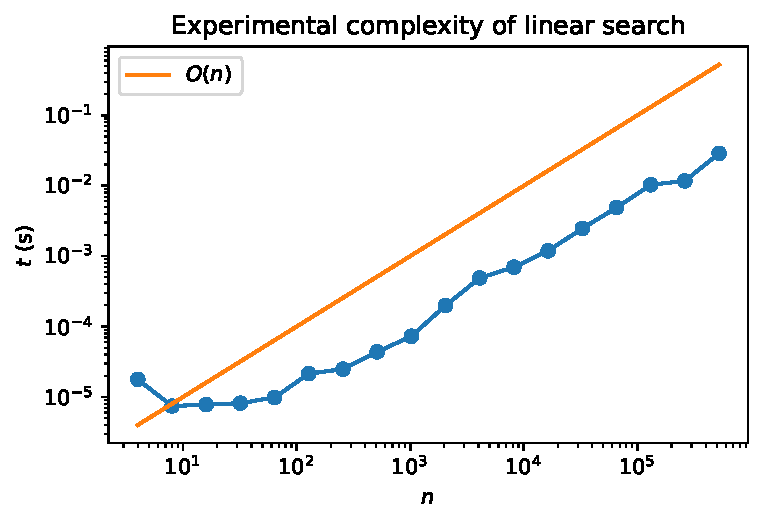
\includegraphics{./complexity_files/figure-pdf/cell-4-output-1.pdf}

}

\end{figure}

The ``experimental noise'' in these plots arises because we don't have
full control over exactly what our computer is doing at any moment:
there are lots of other processes running. Also, it takes a while to
reach the linear regime: there is an overhead associated with starting
the program that represents a smaller fraction of the overall run time
as \(n\) increases.

\hypertarget{better-than-linear}{%
\subsection{Better than linear?}\label{better-than-linear}}

It seems obvious that for search you can't do better than linear: you
have to look at roughly half the items before you should expect to find
the one you're looking for \footnote{\href{https://en.wikipedia.org/wiki/Grover\%27s_algorithm}{Grover's
  algorithm} for search has \(O(\sqrt{n})\) complexity, but there's a
  catch: you need a \emph{quantum computer}, and even then a
  \(\sqrt{n}\) speedup is not going to get you a billion dollars in this
  economy.}. What if the list is \emph{ordered}? Any order will do:
numerical for numbers, or lexicographic for strings. This extra
structure allows us to use an algorithm called
\href{https://en.wikipedia.org/wiki/Binary_search_algorithm}{binary
search} that you may have seen before. The idea is pretty intuitive:
look in the middle of the list and see if the item you seek should be in
the top half or bottom half. Take the relevant half and divide it in
half again to determine which quarter of the list your item is in, and
so on. Here's how it looks in code:

\begin{Shaded}
\begin{Highlighting}[]
\KeywordTok{def}\NormalTok{ binary\_search(x, val):}
    \CommentTok{"""Peform binary search on x to find val. If found returns position, otherwise returns None."""}

    \CommentTok{\# Intialise end point indices}
\NormalTok{    lower, upper }\OperatorTok{=} \DecValTok{0}\NormalTok{, }\BuiltInTok{len}\NormalTok{(x) }\OperatorTok{{-}} \DecValTok{1}

    \CommentTok{\# If values is outside of interval, return None }
    \ControlFlowTok{if}\NormalTok{ val }\OperatorTok{\textless{}}\NormalTok{ x[lower] }\KeywordTok{or}\NormalTok{ val }\OperatorTok{\textgreater{}}\NormalTok{ x[upper]:}
        \ControlFlowTok{return} \VariableTok{None}

    \CommentTok{\# Perform binary search}
    \ControlFlowTok{while} \VariableTok{True}\NormalTok{:}
                
        \CommentTok{\# Compute midpoint index (integer division)}
\NormalTok{        midpoint }\OperatorTok{=}\NormalTok{ (upper }\OperatorTok{+}\NormalTok{ lower)}\OperatorTok{//}\DecValTok{2}

        \CommentTok{\# Check which side of x[midpoint] val lies, and update midpoint accordingly}
        \ControlFlowTok{if}\NormalTok{ val }\OperatorTok{\textless{}}\NormalTok{ x[midpoint]:}
\NormalTok{            upper }\OperatorTok{=}\NormalTok{ midpoint }\OperatorTok{{-}} \DecValTok{1}
        \ControlFlowTok{elif}\NormalTok{ val }\OperatorTok{\textgreater{}}\NormalTok{ x[midpoint]:}
\NormalTok{            lower }\OperatorTok{=}\NormalTok{ midpoint }\OperatorTok{+} \DecValTok{1}
        \ControlFlowTok{elif}\NormalTok{ val }\OperatorTok{==}\NormalTok{ x[midpoint]:  }\CommentTok{\# found, so return}
            \ControlFlowTok{return}\NormalTok{ midpoint}
       
        \CommentTok{\# In this case val is not in list (return None)}
        \ControlFlowTok{if}\NormalTok{ upper }\OperatorTok{\textless{}}\NormalTok{ lower:}
            \ControlFlowTok{return} \VariableTok{None}
\end{Highlighting}
\end{Shaded}

And here's the performance

\begin{Shaded}
\begin{Highlighting}[]
\CommentTok{\# Create array of problem sizes we want to test (powers of 2)}
\NormalTok{N }\OperatorTok{=} \DecValTok{2}\OperatorTok{**}\NormalTok{np.arange(}\DecValTok{2}\NormalTok{, }\DecValTok{24}\NormalTok{)}

\CommentTok{\# Creat array and sort}
\NormalTok{x }\OperatorTok{=}\NormalTok{ np.arange(N[}\OperatorTok{{-}}\DecValTok{1}\NormalTok{])}
\NormalTok{x }\OperatorTok{=}\NormalTok{ np.sort(x)}

\CommentTok{\# Initlise an empty array to capture time taken}
\NormalTok{times }\OperatorTok{=}\NormalTok{ []}

\CommentTok{\# Time search for different problem sizes}
\ControlFlowTok{for}\NormalTok{ n }\KeywordTok{in}\NormalTok{ N:}
    \CommentTok{\# Time search function for finding \textquotesingle{}2\textquotesingle{}}
\NormalTok{    t }\OperatorTok{=} \OperatorTok{\%}\NormalTok{timeit }\OperatorTok{{-}}\NormalTok{q }\OperatorTok{{-}}\NormalTok{n5 }\OperatorTok{{-}}\NormalTok{r2 }\OperatorTok{{-}}\NormalTok{o binary\_search(x[:n], }\DecValTok{2}\NormalTok{)}

    \CommentTok{\# Store average}
\NormalTok{    times.append(t.best)}

\CommentTok{\# Plot and label the time taken for binary search}
\NormalTok{plt.semilogx(N, times, marker}\OperatorTok{=}\StringTok{\textquotesingle{}o\textquotesingle{}}\NormalTok{)}
\NormalTok{plt.xlabel(}\StringTok{\textquotesingle{}$n$\textquotesingle{}}\NormalTok{)}
\NormalTok{plt.ylabel(}\StringTok{\textquotesingle{}$t$ (s)\textquotesingle{}}\NormalTok{)}

\CommentTok{\# Change format on y{-}axis to scientific notation}
\NormalTok{plt.ticklabel\_format(style}\OperatorTok{=}\StringTok{\textquotesingle{}sci\textquotesingle{}}\NormalTok{, axis}\OperatorTok{=}\StringTok{\textquotesingle{}y\textquotesingle{}}\NormalTok{, scilimits}\OperatorTok{=}\NormalTok{(}\DecValTok{0}\NormalTok{,}\DecValTok{0}\NormalTok{))}
\NormalTok{plt.title(}\StringTok{"Experimental complexity of binary search"}\NormalTok{)}
\NormalTok{plt.show()}
\end{Highlighting}
\end{Shaded}

\begin{figure}[H]

{\centering 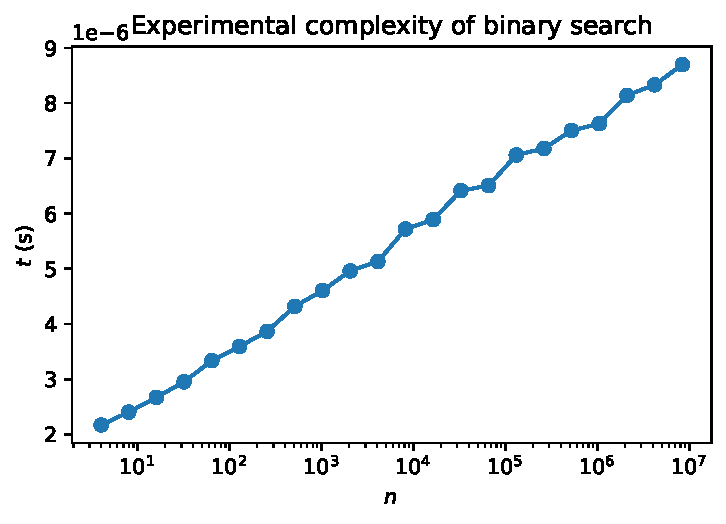
\includegraphics{./complexity_files/figure-pdf/cell-6-output-1.pdf}

}

\end{figure}

Note the axes: the plot is linear-log, so the straight line indicates
\emph{logarithmic} growth of complexity. This makes sense: if the length
is a power of 2 i.e.~\(n=2^p\), we are going to need \(p\) bisections to
locate our value. The complexity is \(O(\log n)\) (we don't need to
specify the base as overall constants don't matter).

This strategy of getting better than linear scaling

Intro to recursion

\hypertarget{from-quadratic-to-linear}{%
\section{From quadratic to linear}\label{from-quadratic-to-linear}}

Of course, it is still worth

Example of checking pairs

A major goal in algorithm design

\hypertarget{examples-of-different-complexities}{%
\section{Examples of different
complexities}\label{examples-of-different-complexities}}

Summary of asymptotic notation

XKCD plots

\hypertarget{space-vs.-time-complexity}{%
\section{Space vs.~time complexity}\label{space-vs.-time-complexity}}

\hypertarget{back-to-multiplication-divide-and-conquer}{%
\section{Back to multiplication: divide and
conquer}\label{back-to-multiplication-divide-and-conquer}}

\href{https://en.wikipedia.org/wiki/Karatsuba_algorithm}{Karatsuba
algorithm} nice story

\href{http://www.cs.ru/personal/karatsuba/divcen.pdf}{Karatsuba's
account}

Karatsuba (1995) contains a nice account of the discovery of his
algorithm (\href{http://www.cs.ru/personal/karatsuba/divcen.pdf}{online
version})

Karatsuba algo

Big O

\href{https://www.sortvisualizer.com/}{Visualization of sorting
algorithms}

Simple example from Leetcode

Analaysis of algorithms

Example of finding a unique item in list

Nice examples from Garth Wells

https://github.com/CambridgeEngineering/PartIA-Computing-Michaelmas/blob/main/11\%20Complexity.ipynb

Examples of multiplication

Breadth first and depth first

Importance of choosing a data structure to match algorithm

Examples: queue in Wolff. Was there a Numpy-ish way to do this faster?
Priority queue in waiting time algo

FFT uses

https://en.wikipedia.org/wiki/Orthogonal\_frequency-division\_multiplexing

Needleman-Wunsch

Examples

\begin{enumerate}
\def\labelenumi{\arabic{enumi}.}
\tightlist
\item
  Multiplication
  \href{https://en.wikipedia.org/wiki/Multiplication_algorithm\#Karatsuba_multiplication}{Karatsuba}
\item
  Binary search
\item
  Linear algebra
\item
  Sorting
\item
  FFT
\item
  Taking powers (SICP). What is \(n\) in this case?
\item
  Euclidean algorithm (GCD) (SICP)
\end{enumerate}

References. Nature of computation, grokking algos

Insertion in a list etc.

\bookmarksetup{startatroot}

\hypertarget{linear-algebra}{%
\chapter{Linear algebra}\label{linear-algebra}}

Krylov subspaces

SVD and quantum mechanics. Quantum entanglement.

Image compression using SVD

http://timbaumann.info/svd-image-compression-demo/

Trebst has nice Einstein example

PCA for big data

\bookmarksetup{startatroot}

\hypertarget{divide-and-conquer}{%
\chapter{Divide and Conquer}\label{divide-and-conquer}}

FFT. Use split step as illustration Matrix multiplication

\bookmarksetup{startatroot}

\hypertarget{dynamic-programming}{%
\chapter{Dynamic Programming}\label{dynamic-programming}}

\bookmarksetup{startatroot}

\hypertarget{automatic-differentiation}{%
\chapter{Automatic Differentiation}\label{automatic-differentiation}}

Karpathy's micrograd
\href{http://neuralnetworksanddeeplearning.com/}{Michael Nielsen's book}

\bookmarksetup{startatroot}

\hypertarget{summary}{%
\chapter{Summary}\label{summary}}

In summary, this book has no content whatsoever.

\bookmarksetup{startatroot}

\hypertarget{references}{%
\chapter*{References}\label{references}}
\addcontentsline{toc}{chapter}{References}

\markboth{References}{References}

\hypertarget{refs}{}
\begin{CSLReferences}{1}{0}
\leavevmode\vadjust pre{\hypertarget{ref-jacobs1981multi}{}}%
Jacobs, Laurence, and Claudio Rebbi. 1981. {``Multi-Spin Coding: A Very
Efficient Technique for Monte Carlo Simulations of Spin Systems.''}
\emph{Journal of Computational Physics} 41 (1): 203--10.

\leavevmode\vadjust pre{\hypertarget{ref-kapfer2013sampling}{}}%
Kapfer, Sebastian C, and Werner Krauth. 2013. {``Sampling from a
Polytope and Hard-Disk Monte Carlo.''} In \emph{Journal of Physics:
Conference Series}, 454:012031. 1. IOP Publishing.

\leavevmode\vadjust pre{\hypertarget{ref-karatsuba1995complexity}{}}%
Karatsuba, Anatolii Alexeevich. 1995. {``The Complexity of
Computations.''} \emph{Proceedings of the Steklov Institute of
Mathematics-Interperiodica Translation} 211: 169--83.

\leavevmode\vadjust pre{\hypertarget{ref-krauth1998introduction}{}}%
Krauth, Werner. 1998. {``Introduction to Monte Carlo Algorithms.''} In
\emph{Advances in Computer Simulation}, 1--35. Springer.

\leavevmode\vadjust pre{\hypertarget{ref-krauth2006statistical}{}}%
---------. 2006. \emph{Statistical Mechanics: Algorithms and
Computations}. Vol. 13. OUP Oxford.

\leavevmode\vadjust pre{\hypertarget{ref-mackay2003information}{}}%
MacKay, David JC. 2003. \emph{Information Theory, Inference and Learning
Algorithms}. Cambridge university press.

\leavevmode\vadjust pre{\hypertarget{ref-widom1966random}{}}%
Widom, B. 1966. {``Random Sequential Addition of Hard Spheres to a
Volume.''} \emph{The Journal of Chemical Physics} 44 (10): 3888--94.

\end{CSLReferences}



\end{document}
